\documentclass[letterpaper]{article}
\usepackage{amssymb}
\usepackage{fullpage}
\usepackage{changepage}
\usepackage{amsmath}
\usepackage{epsfig,float,alltt}
\usepackage{psfrag,xr}
\usepackage[T1]{fontenc}
\usepackage{url}
\usepackage{pdfpages}
\usepackage{epstopdf}
\usepackage[framed,numbered,autolinebreaks,useliterate]{mcode}

%\includepdfset{pagecommand=\thispagestyle{fancy}}
\author{Fan Bu, Feng Zhou, Yi Yang}
\title{ME 552 Lab 03 Report}

\begin{document}
\date{10/15/2016}
\maketitle

\newcommand{\trace}{\mathrm{trace}}
\newcommand{\real}{\mathbb R}  % real numbers  {I\!\!R}
\newcommand{\nat}{\mathbb N}   % Natural numbers {I\!\!N}
\newcommand{\cp}{\mathbb C}    % complex numbers  {I\!\!\!\!C}
\newcommand{\ds}{\displaystyle}
\newcommand{\mf}[2]{\frac{\ds #1}{\ds #2}}
\newcommand{\spanof}[1]{\textrm{span} \{ #1 \}}
\newcommand{\sol}[0]{\textbf{Solution: }}
\newcommand{\pf}[0]{\textbf{Proof:}}
\newcommand{\rme}[0]{\textrm{e}}
\newcommand{\Null}[1]{\textrm{Null}\{#1\}}
\parindent 0pt
%%%%%%%%%%%%%%%%%%%%%%%%%%%%%%%%%%%%%%%%%%%%%%%%%%%%%%%%%%%%%%%%%%%%%%%%%%%%%%%
% Solution for Question 1 begins here - by Yi Yang
%%%%%%%%%%%%%%%%%%%%%%%%%%%%%%%%%%%%%%%%%%%%%%%%%%%%%%%%%%%%%%%%%%%%%%%%%%%%%%%
\section*{Question 1}
\subsection*{(a)}
Study the AMC servo-amplifier datasheet and identify the functionality of op-amps U1, U3 and U4 qualitatively and quantitatively.\\

The circuits for U1 is shown as:

\begin{figure}[H]
	\centering
	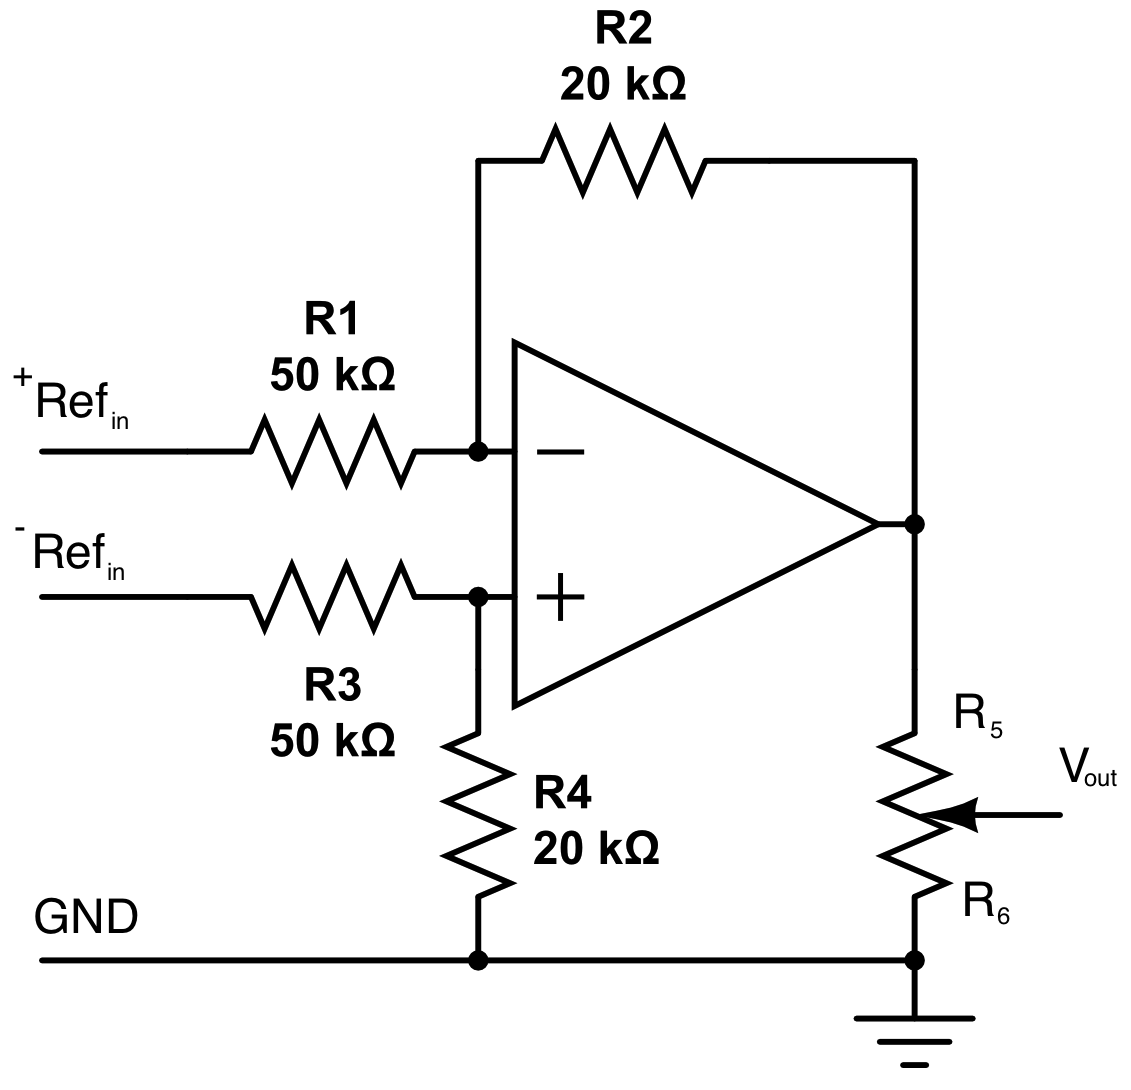
\includegraphics[scale=0.15]{q1a_u1.png}
	\caption{Unit 1 circuits in AMC circuits}
\end{figure}
U1 is a difference circuit between $^-Ref$ and $^+Ref$ with a gain that is regulated by a potentiometer.
$$ V_{out} = \left( \frac{R_6}{R_5+R_6} \right) \left( \left(1 + \frac{R_2}{R_1} \right) \left( \frac{R_4}{R_3+R_4} \right) (^-Ref) - \left( \frac{R_2}{R_1} \right) (^+Ref) \right) $$
$$ V_{out} = \left( \frac{R_6}{R_5+R_6} \right) \left( \left(1+ \frac{20}{50} \right) \left( \frac{20}{50+20} \right)(^-Ref) - \left( \frac{20}{50} \right) (^+Ref) \right) $$
The circuit for U3 is pictured as follows:\\
U3 is a inverting amplifier and it is tunned by the potentiometer.
$$U3_{out} = - \left( \frac{R_3 + R_4}{R_4} \right) \left( \frac{R_2}{R_1} \right) Ref_{gain} $$
$$U3_{out} = - \left( \frac{R_3 + R_4}{R_4} \right) \left( \frac{10}{5} \right) Ref_{gain} $$
\begin{figure}[H]
	\centering
	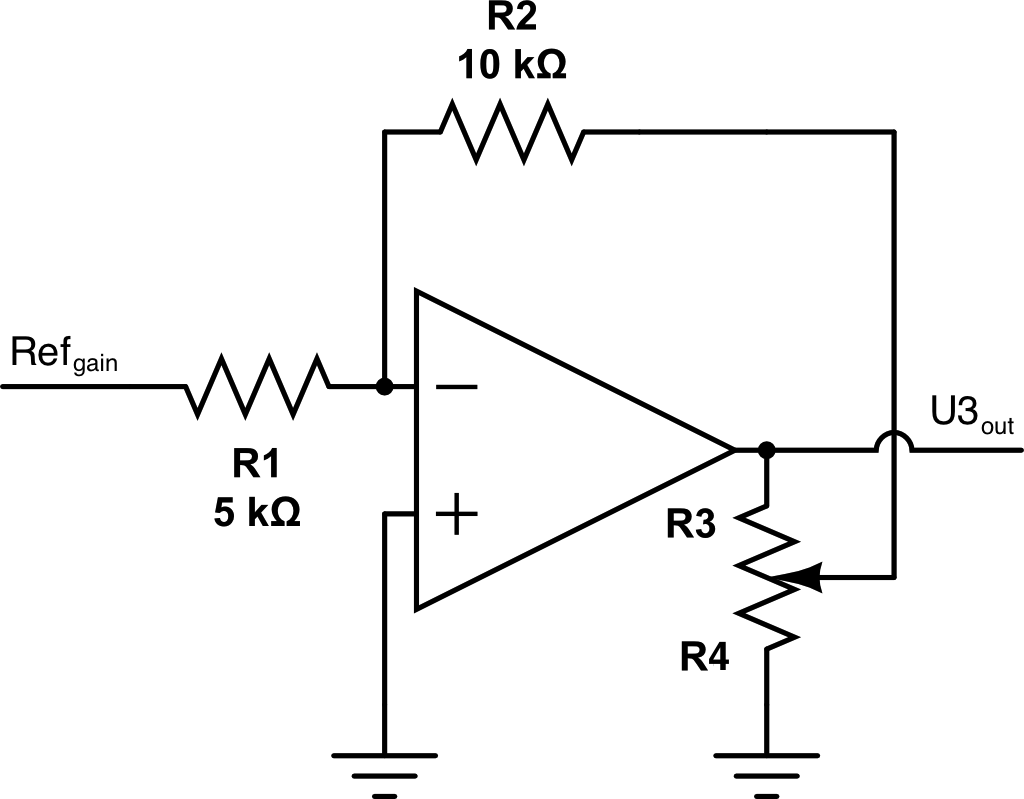
\includegraphics[scale=0.15]{q1a_u3.png}
	\caption{Unit 3 circuits in AMC circuits}
\end{figure}
The circuit for U4 is shown as:
\begin{figure}[H]
	\centering
	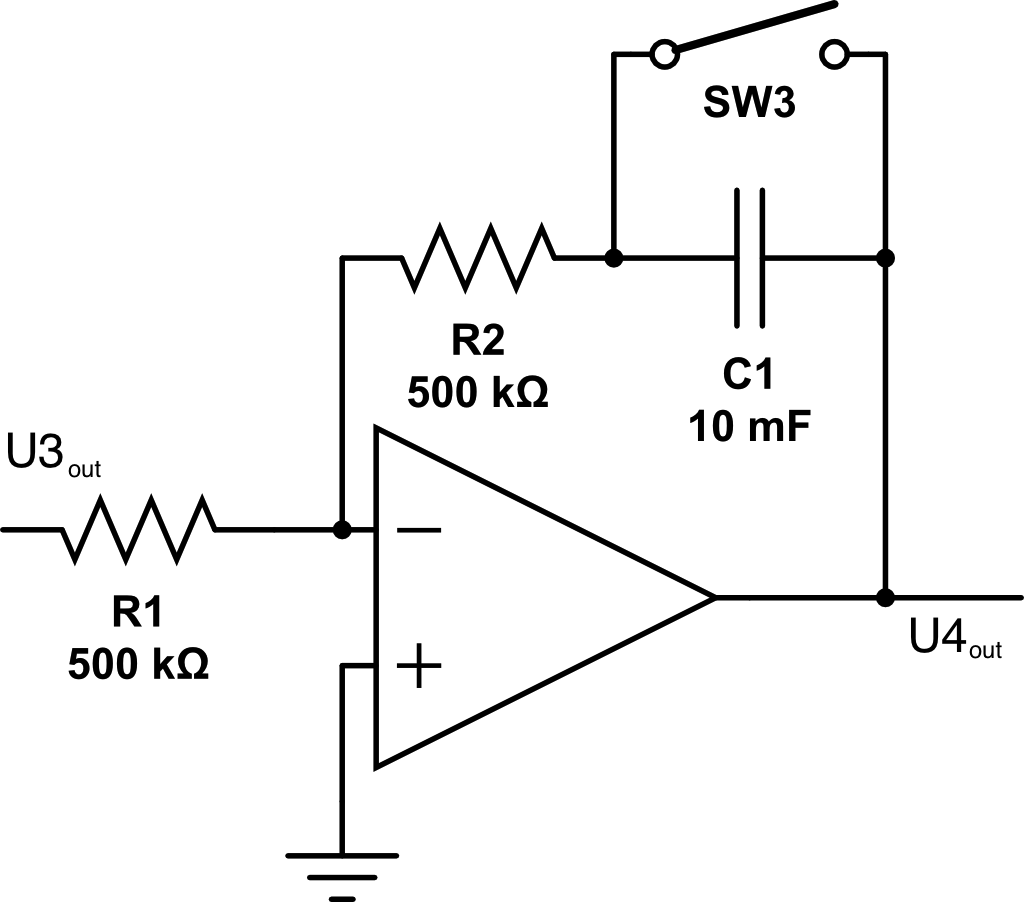
\includegraphics[scale=0.15]{q1a_u4.png}
	\caption{U 4 circuit in AMC circuit}
\end{figure}
As the circuit shown above, when switch 3 is open, U3 will serve as an inverting integrator with a proportional gain, when switch is closed, the circuit will serve as an inverting circuit.
$$U4_{out} = - \left( \frac{1}{R_1} \right) \left( R_2 + \frac{1}{C_1s} \right) U3_{out} $$
$$U4_{out} = - \left( \frac{1}{500} \right) \left( 500 + \frac{1}{0.01s} \right) U3_{out} $$

\subsection*{(b)}
This resistor serves to isolate the current that flows through this section of the circuit to the outer load circuit. The current sensor transform the current signal into a voltage signal and output this signal through the current monitor P1-8. Thus, to monitor the scale of the current, we can simply connect a voltage-meter or an A/D converter to this signal, the scale of the voltage we measure simply stands for the scale of the current. When this output shortcut the ground, this 10K resistor may serve as a protector resistance that won't cause too large current through this circuit branch. Moreover, since the input resistance of the voltage-meter and the A/D converter are all extremely large, the 10K resistor will not affect the accuracy of measurement.

\subsection*{(c)}
Refer to the motor datasheet and determine the \textbf{maximum continuous current}, provide a physical and mathematical justification for the maximum continuous current value that you are proposing. How does this compare with the \textbf{maximum rated current} listed in the datasheet. Attempt a similar educated estimate of \textbf{maximum intermittent} or \textbf{noncontinuous, peak current} that the motor can handle. Explain the datasheet's and/or your interpretation of maximum intermittent current.\\

Looking up the datasheet of Pittman 9237S011 motor, we see the maximum winding temperature for the motor is $155 ^\circ C$, and a thermal impedance is $11.2 \, \tfrac{^\circ C}{W}$.  Assuming a room temperature of $25^\circ$C, the motor's temperature can only increase by $130^\circ$C before overheating. With these values and the motor's internal resistance of $1.85 \, \Omega$, we can solve for the maximum continuous current:

$$130 = 11.2\cdot i_{cont}^2 \cdot 1.85$$
$$i_{cont} = 2.5048 \,A$$

With this current and the given torque constant we can then calculate the maximum continuous torque:

$$T_{m} = k_{t} \cdot i_{cont} = 4.24\times 10^{-2}\times 2.5048 = 10.6\times 10^{-2}\, Nm$$

We observed that this value is less conservative than the continuous torque ratings given on the datasheet which is $8.1 \times 10^{-2}\, Nm$, hence the max continuous current should be $1.92 A$, and the temperature rise would be $75^\circ$C above ambient. This means that at the max torque given by the data sheet, the motor would be well under the temperature limit. It's possible that the given value is either based on a safety factor to prevent overheating, or there are other modes of breakdown that can result from higher currents. If the lower limit is based on temperature, then we should be able to use slightly higher currents given that we are running for short periods.\\
The motor's data sheet lists a peak current rating of 13.0 $A$ and a stall torque of 0.54 $N \cdot m$. With this torque value and the given torque constant (4.24$\times 10^{-2} \tfrac{(N \cdot m)}{A}$), the peak current should be:
$$i_{peak} = \dfrac{T_{stall}}{k_{t}} = \dfrac{0.54}{4.24\times 10^{-2}} = 12.74 \,A$$
This is less than the given rating for peak current. At this peak current limit, the motor dissipates approximately 300 W.  If the system were allowed to run at this current, and assuming that the motor does not fail in some way, it would reach a steady state temperature of:
$$P = i_{peak}^2 \cdot R_{m} = 12.74^2 \times 1.85 = 300.269 \,W$$
$$\Delta Temp = P \cdot R_{t} = 300.269 \times 11.2 = 3363.0128  \,{^\circ}C$$ 
It is obvious that our motor can not operate normally under this heat loads for a long period and we can use an exponential model to approximate the transient process of heat dissipation in the inner circuit of our motor. The thermal time constant is given as $13.8(828)$ min(seconds). Hence we can plot the results in the figure below and motor will break down because of overheat after 32.4 seconds.
\begin{figure}[H]
	\centering
	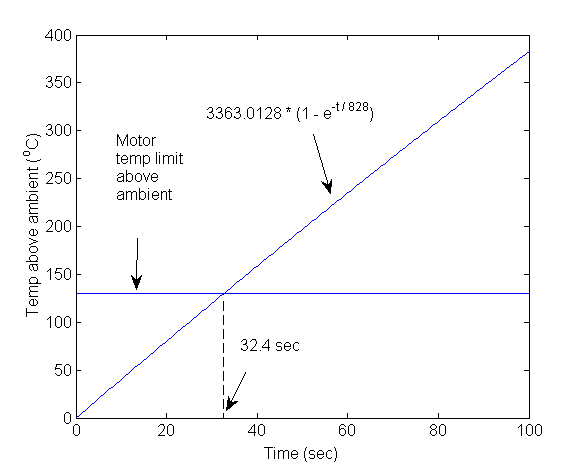
\includegraphics[scale=0.5]{temperature.png}
	\caption{Motor temperature over time in intermittent mode}
\end{figure}

\subsection*{(d)}
Based on the Servo-Amp Datasheet and Part3 of Lab3 Instructions, what are the \textbf{maximum continuous} and \textbf{intermittent current} values that op-amp can output to the motor? Provide a clear and detailed explanation. Explain the Servo-Amp datasheet's interpretation of intermittent current.\\

Refering to the datasheet of 12A8E servo amplifier, the maximum continuous and peak currents are $\pm 6A$ and $\pm 12A$, respectively (from the data sheet) and the servo amplifier includes a potentiometer used to reduce both the continuous and peak currents while maintaining a 1:2 relationship between them. The lab instructions specify that the potentiometer should be adjusted so that the current limits will be $\pm 3A$ and $\pm 6A$.  The continuous current limit can be further reduced, without affecting the peak current, by connecting a current limiting resistor between pins P1-10 and P1-2 on the servo-amp(explained in the datasheet). Assuming the adjustment on the current limiting potentiometer was done correctly, the servo-amp should be capable of sending $\pm 3A$ continuously and $\pm6A$ intermittently to the motor. The continuous current limit from the servo-amp is greater than the continuous current rating of the motor, so we must adjust the output of maximum continuous current of op-amp to make sure the safety of motor.
The datasheet for the servo-amp specifies a peak current of $\pm12 A$ for a maximum of 2 seconds. This means this maximum current can maintain for less than 2 seconds before the circuit is switched to make current range between -12 and 12 A. A smaller switch magnitude will be allowed to maintain for less time period (i.e. switching from 0 A to +12 A will only be held for 1 second before the current begins falling). The primary concern with maintaining high currents is overheating, and the servo-amp has a much lower temperature limit than the motor (65 $^\circ$C vs 155 $^\circ$C), as well as a much smaller thermal time constant than the motor.  This is why the peak current can not be maintained for long, the maximum temperature would be exceeded very quickly and the servo-amp's internal safeties would shut it off. As an example, in the thermal model for the motor at peak current (which is lower than the 6 A rating of the servo-amp), 65 $^\circ$C was reached in only 9.8 seconds. Of course, the servo-amp has different thermal properties than the motor, so that specific value is not accurate. However, the basic idea is valid: the servo-amp is capable of passing a lot of current, and has a lower temperature limit than the motor, so there is a danger of it overheating if high currents are maintained. Luckily, the servo-amp has built in safeties, such as a thermal shut-off.

\subsection*{(e)}
What command \textbf{saturation limit} would you include in your labview controller? How would you ensure a safe operation of all the hardware hardware involved in this experiment?\\

We have seen in the section (c) that the motor has a continuous and peak current limits of 2.5 A and 12.74 A, and the servo-amp  has current limits of 3 A and 6 A, respectively. Within our LabView controller we chose to implement saturation limits of $\pm6$ A so that we could take advantage of the peak current capability of the servo-amp and motor. We considered setting a saturation limit based on the motor's continuous current limit of 2.5 A, but felt that might have a negative effect on the transient response of the motor. Also, we knew that the servo-amp has built in mechanisms to prevent the current from remaining at the peak value. That is to say it automatically lowers it after at most two seconds. Additionally, as we were tuning our LabView controller, we monitored a waveform graph of the attempted output of the controller. This allowed us to adjust our gain values not just for system stability, but also to keep the attempted output within safe limits. Given more resources, we could have implemented more safety measures. For example, we could add a fuse to set a current limit that is a little under the continuous current limit of the motor. This would protect the system from high currents for prolonged period of time, but still allow for short bursts of higher current during transient conditions.

\section*{Question 2}
\subsection*{(a)}
We can use figure \ref{q2_1} to model the inner structure of a DC motor dynamic system, the torque is proportional to the input current. Also, we omit the effects of Coulomb friction and assume the load torque equals 0, we can get:\\
$$J\frac{d\omega }{dt}+B\omega =K_tI$$
From the equation we obtained, let us do Laplace Transform, assuming input is the current, output is angular velocity, we can get:\\
$$\frac{\omega (s)}{I(s)}=\frac{K_t}{Js+B} \text{ or } \mf{\theta(s)}{I(s)} = \mf{K_t}{s(Js+B)}$$
If we consider the effects of driver circuits (op-amp), we can model the overall system dynamics as:\\
$$V_s - K_b\mf{d\theta}{dt} = iR + L\mf{di}{dt}$$
$$\mf{\theta(s)}{V_s(s)} = \mf{K_t}{s\left[\left(Js+B\right)\left(Ls+R\right)+K_bK_t\right]}$$
$$\mf{\theta(s)}{I(s)} = \mf{K_t}{s\left(Js+B\right)}$$
From the equation above, we can get following table from datasheet.\\
\begin{center}
    \begin{tabular}{ | l | l | l | p{5cm} |}
    \hline
    Rotor Inertia $(kg\cdot m^2)$ & $J$ & 8.5e-6 \\ \hline
    Damping Constant $(N\cdot m\cdot s)$ & $B$ & 9.7e-4\\ \hline
    Torque Constant $(N\cdot m/A)$ & $K_t$ & 4.24e-2 \\ \hline
    Coulomb Friction Torque Constant $(N\cdot m)$ & $T_f$ & 5.6e-3 \\ \hline
    \end{tabular}
\end{center}
\begin{figure}[H]
	\centering
	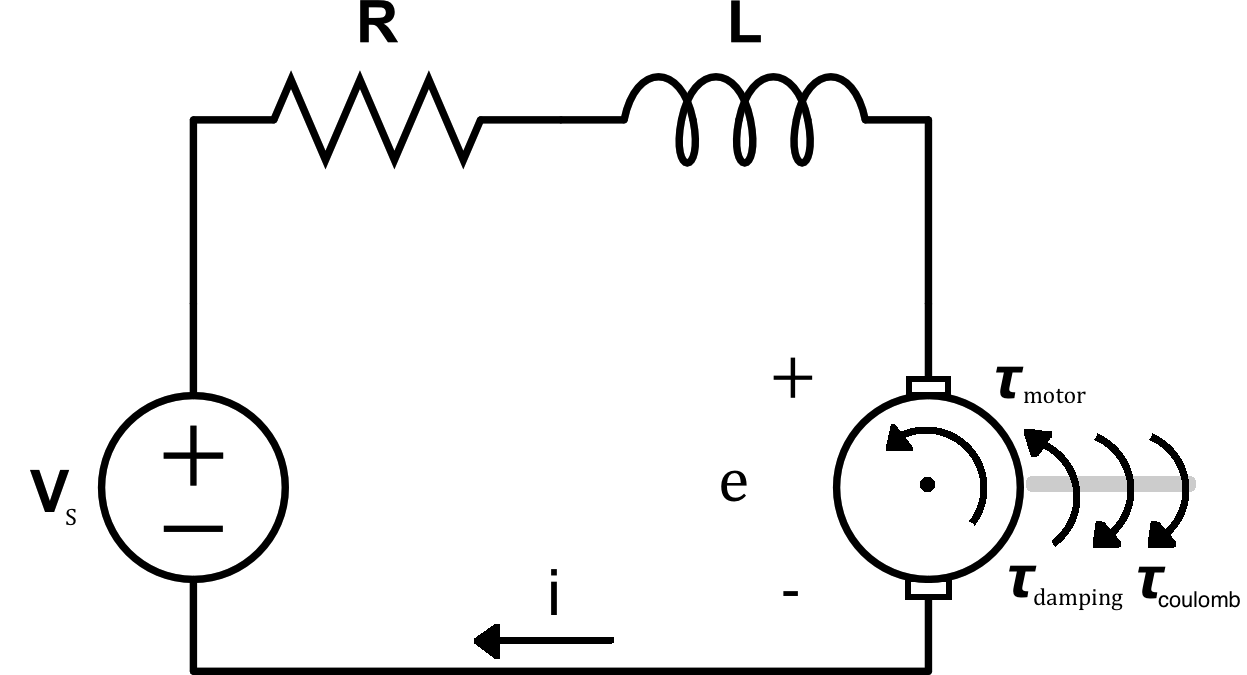
\includegraphics[width = 10cm, height = 6cm]{dcmotor.png}
	\caption{Equivalent circuits of combined driver and dc motor}
	\label{q2_1}
\end{figure}
\subsection*{(b)}
First of all, under current control mode, we start to run our motor with a step input (as the ratio of command voltage and current is 1, for example we can provide a step input with $0.5$ Volts command voltage to get a $0.5A$ current into the motor). Below is the mathematical model of our DC motor model.\\
$$\omega (s)=\frac{K_t}{Js+B}=\frac{K_t/J}{s+B/J}$$
From the equation above, when we do not have the motor datasheet, in order to get the model we need for our experiment, we need to identify the $K_t/J$ and $B/J$. \\
Now we store our step response data (input is current and output is angular velocity ) in file then import them into MATLAB. In MATLAB, first let us type "ident" to open the System Identification Toolbox, shown as the GUI in Figure \ref{q2_b_1}.\\
\begin{figure}[htb]
\begin{center}
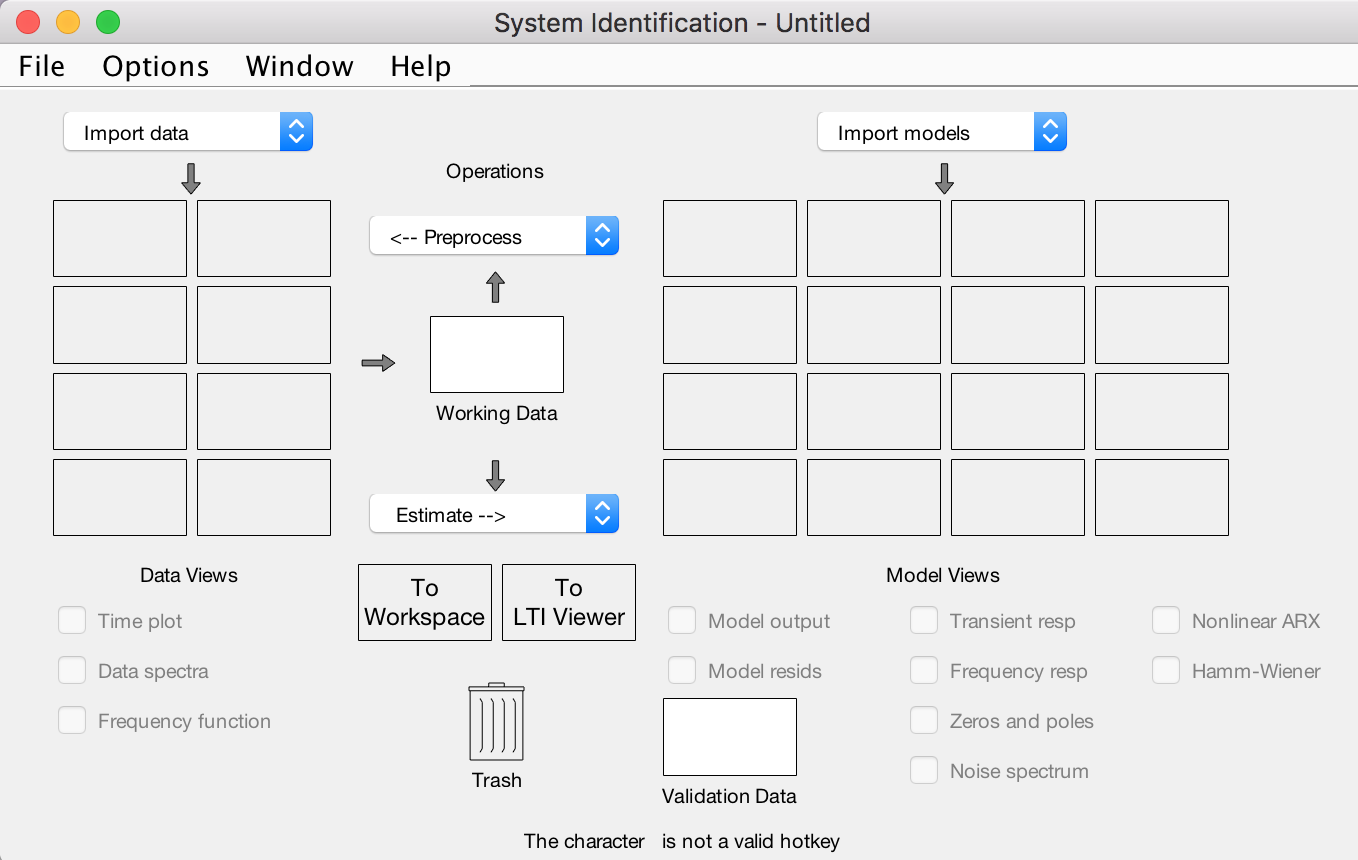
\includegraphics[width = 10cm]{q2_b_1.png}
\caption{Identification Toolbox GUI}
\label{q2_b_1}
\end{center}
\end{figure}
For the next step, we will use MATLAB system identification GUI to identify our system. Then, we may import the given experimental data in one of the left boxes using our time-domain data.
After import our data, we should define the numbers of pole and zero of our transfer function. As we had derived our transfer function, we know we have 1 pole and 0 zero. After configuration, we click estimate, as shown in Figure \ref{q2_b_2}.\\
\begin{figure}[H]
\begin{center}
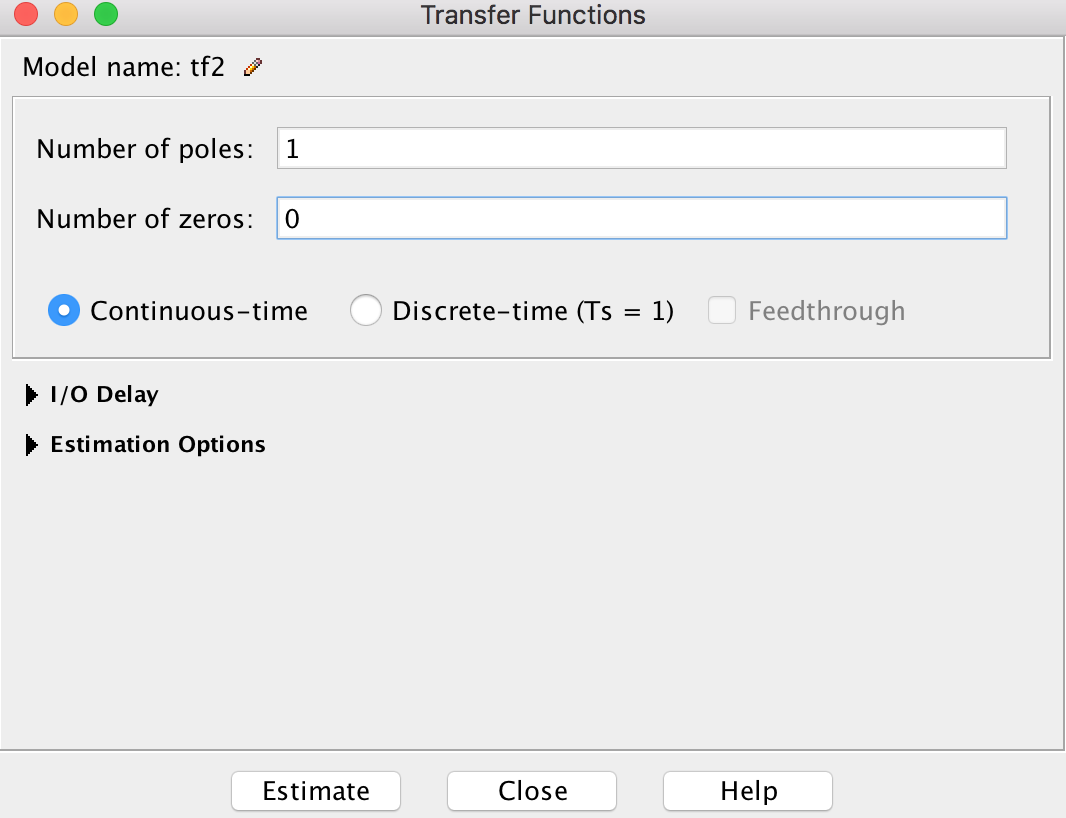
\includegraphics[width = 10cm]{q2_b_2.png}
\caption{Identification Toolbox setting}
\label{q2_b_2}
\end{center}
\end{figure}
And after MATLAB's estimation, we could see that our system is already successfully identified, which is displayed in one of the right boxes, shown in Figure \ref{q2_b_3}.\\
\begin{figure}[H]
\begin{center}
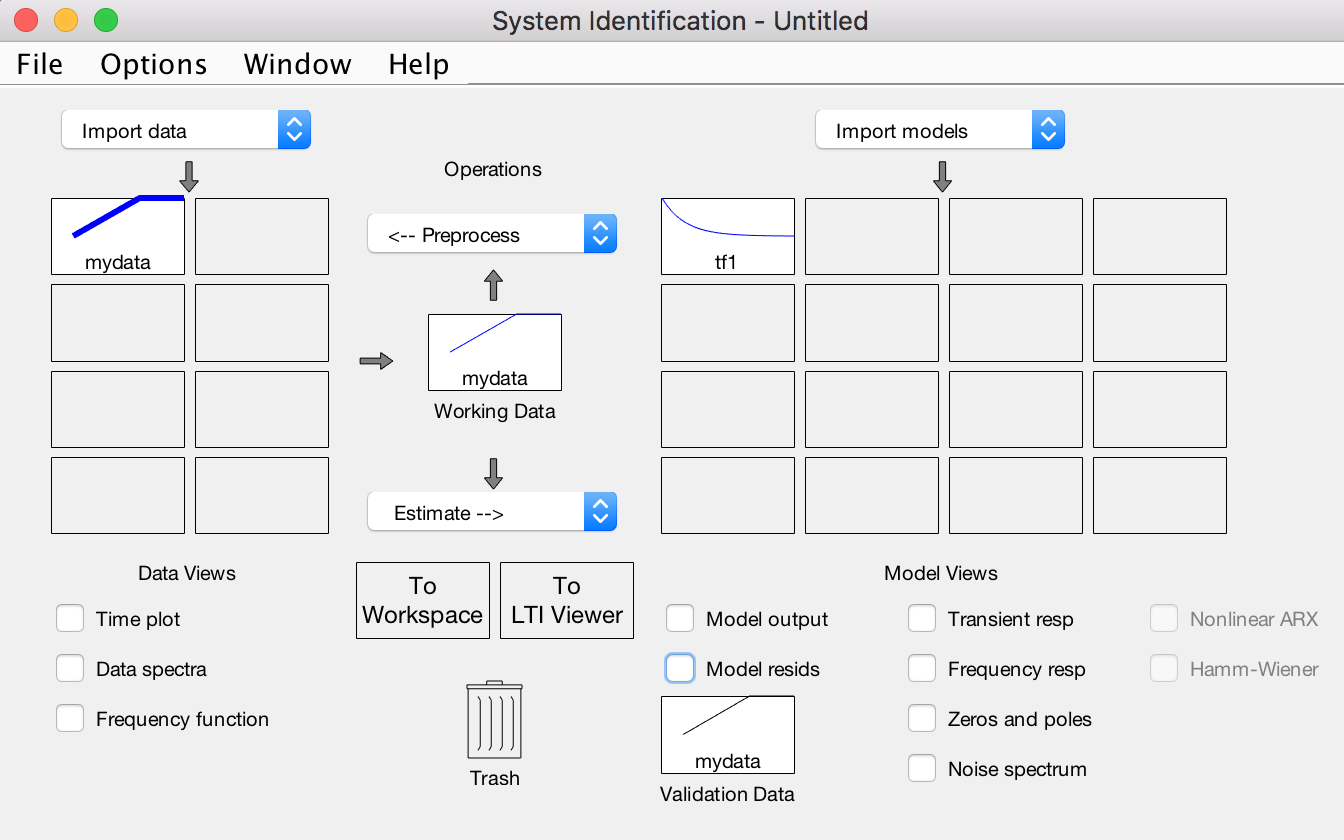
\includegraphics[width = 10cm]{q2_b_3.png}
\caption{Identification Toolbox GUI}
\label{q2_b_3}
\end{center}
\end{figure}
Double click the "tf1" in the right box we can see the transfer function of our system. Finally we compare it with 
$$\Omega (s)=\frac{K_t}{Js+B}=\frac{K_t/J}{s+B/J}$$
By this method, we can obtain the tuned parameters for our system without motor datasheet. Note that instead of resorting to matlab identification tools, we can also directly design some nonlinear regression experiments to optimize experiment data, using the optimized data to approximate the optimal parameters for our system, we think these procedure is highly time-consuming, so we decide to skip some detailed operations and directly plug parameters obtained from datasheet to our system model for controller design in the next step.
%%%%%%%%%%%%%%%%%%%%%%%%%%%%%%%%%%%%%%%%%%%%%%%%%%%%%%%%%%%%%%%%%%%%%%%%%%%%%%%%%
%%%% Fill in contents of Question 2 here
%%%%%%%%%%%%%%%%%%%%%%%%%%%%%%%%%%%%%%%%%%%%%%%%%%%%%%%%%%%%%%%%%%%%%%%%%%%%%%%%%
\section*{Question 3}
We constructed the a \textbf{model} represented as Simulink block shown below, the \textbf{transfer function} between $V_{ref}$ and Motor Angle, and $V_{ref}$ and Motor velocity is derived in Question 2 and we omit its reformulation here. The overall \textbf{Simulink} model and the \textbf{MATLAB file} containing all system parameters are listed below.
The following figure shows the overall model of DC motor servo system for both velocity and position control.
\begin{figure}[H]
	\centering
	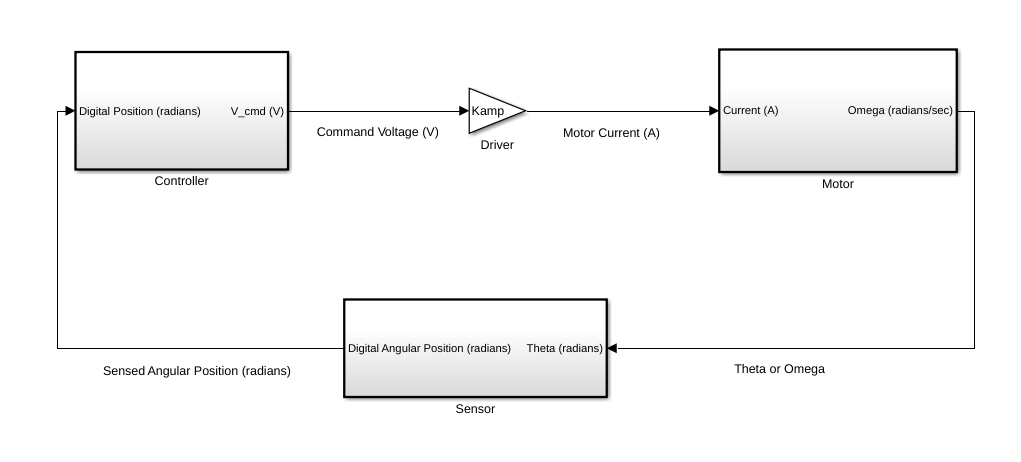
\includegraphics[scale=0.36]{motorServoSystem.png}
	\caption{Overall DC motor system}
	\label{q3_1}
\end{figure}
The DC motor dynamic subsystem is shown below, we will use a piecewise function to model the coulomb friction to the rotor. Coulomb friction torque is modelled as:
\[T_{Coulomb} = \begin{cases} 
      T_f & \omega\geq 1\times10^{-6} \\
      \mf{\omega}{1\times 10^{-6}}\cdot T_f & -1\times 10^{-6} < \omega < 1\times 10^{-6} \\
      -T_f & \omega \leq 1\times 10^{-6} 
   \end{cases}
\]
Where Coulomb friction torque is $T_f = 5.6\times 10^{-3}$ [Nm] in datasheet.
\begin{figure}[H]
	\centering
	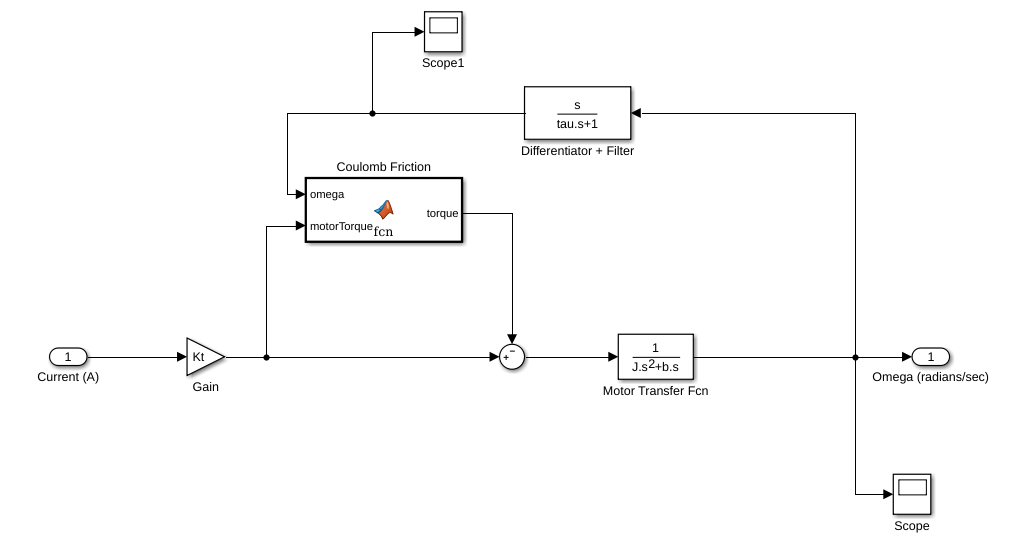
\includegraphics[scale=0.4]{motorSubsystem.png}
	\caption{DC motor subsystem}
	\label{q3_2}
\end{figure}
The optical encoder (see figure \ref{q3_3}) was modeled as a quantizer with the interval size equal to $2\pi/2000$ was used to simulate the effects of the ADC, the interval size is pre-determined in the instruction sheet.

\begin{figure}[H]
\begin{center}
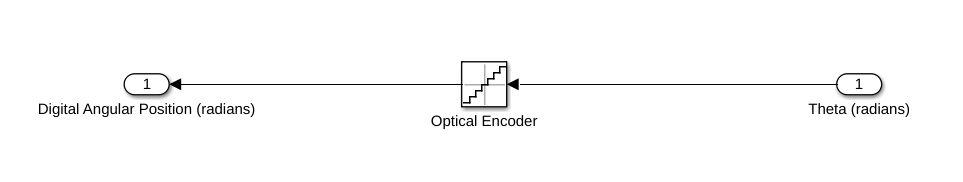
\includegraphics[scale = 0.36]{SensorSubsystem.png}
\caption{The Optical Encoder Subsystem}
\label{q3_3}
\end{center}
\end{figure}
The Servo Amplifier was treated as a gain equal to 1 due to its high bandwidth (2.5 kHz). It can be seen in figure \ref{q3_1}. We first try to tune the PID controller of velocity controller and then decide the PID gain of the position controller. The Simulink module for velocity controller is shown in \ref{q3_4}. The Simulink module for position controller is shown in \ref{q3_5}.
\begin{figure}[H]
	\centering
	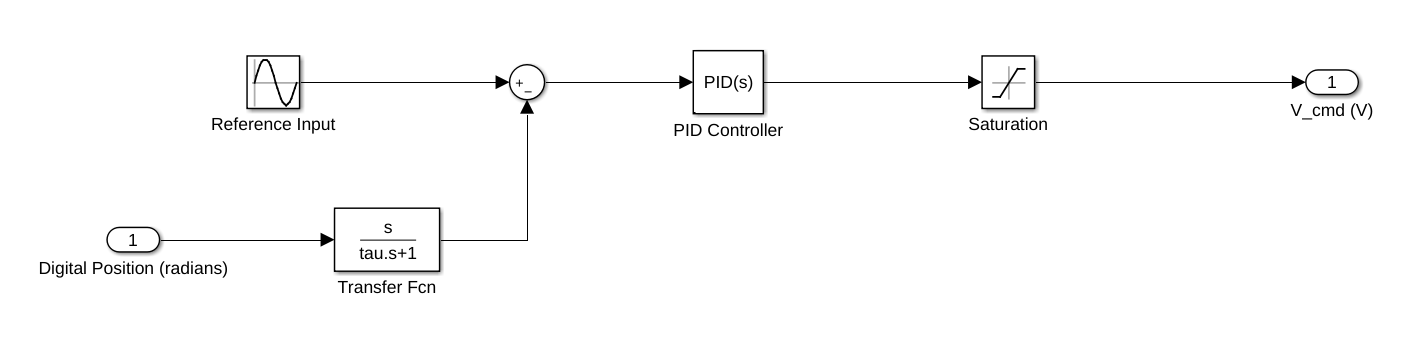
\includegraphics[scale=0.32]{velocityControlSubsystem.png}
	\caption{Velocity controller subsystem}
	\label{q3_4}
\end{figure}
\begin{figure}[H]
	\centering
	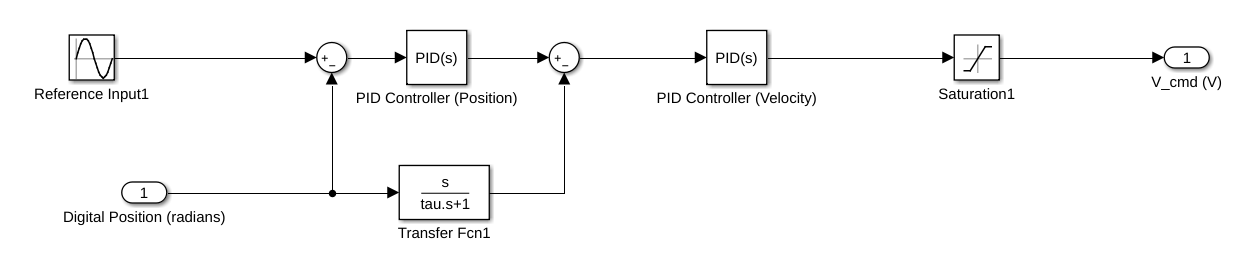
\includegraphics[scale=0.36]{PositionControlSubsystem.png}
	\caption{Position controller subsystem}
	\label{q3_5}
\end{figure}
We will add a saturation module to make sure the current limit will not overpass the maximum peak current of the servo-amp which is $6A$. We see that we calculated a value of $1.92$ A to be the maximum continuous winding current in the DC motor, so we must make sure that the current over $1.92$ A will not last for a long period.\\

The cascaded P/PI controller (see figure \ref{q3_7}) is one of the most commonly used controller structures in motion control systems. It is simple and has a systematic tuning procedure. This configuration allowed us to reuse the velocity controller within our position controller.\\

\begin{figure}[H]
\begin{center}
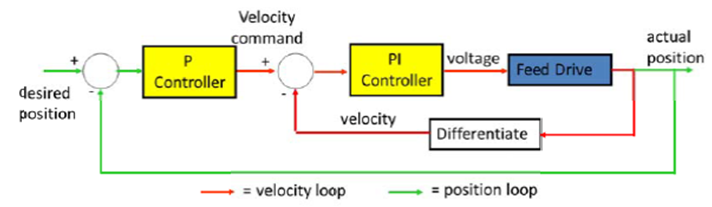
\includegraphics[width = 14 cm]{q3_7}
\caption{Basic Structure of P/PI Controller}
\label{q3_7}
\end{center}
\end{figure}

This design consists of two cascaded loops. The inner one is the velocity loop. It is a PI controller which aims to ensure that the velocity command is tracked accurately. It is surrounded by the outer position loop which is a P controller that ensures the desired reference point is achieved. Having both loops makes it easy to deal with each loop one at a time. The first step is to optimize the PI controller, achieving the best performance in the velocity loop, and then tune the P controller to ensure position tracking performance.\\

Before we began tuning, we needed to know the overall system dynamics, which provide essential information to guide the tuning process. Frequency response was used to analyze the velocity loop based on different values of the time constant, $\tau$. The following figures (\ref{q3_8}, \ref{q3_9} and \ref{q3_10}) show Bode diagrams for the transfer functions of open-loop ($G_{OL}$), close-loop ($G_{CL}$), input disturbance rejection ($G_{di}$), and output disturbance rejection ($G_{do}$) with $\tau = 0.05, 0.1, \text{and } 1$, respectively.
\begin{figure}[H]
\begin{center}
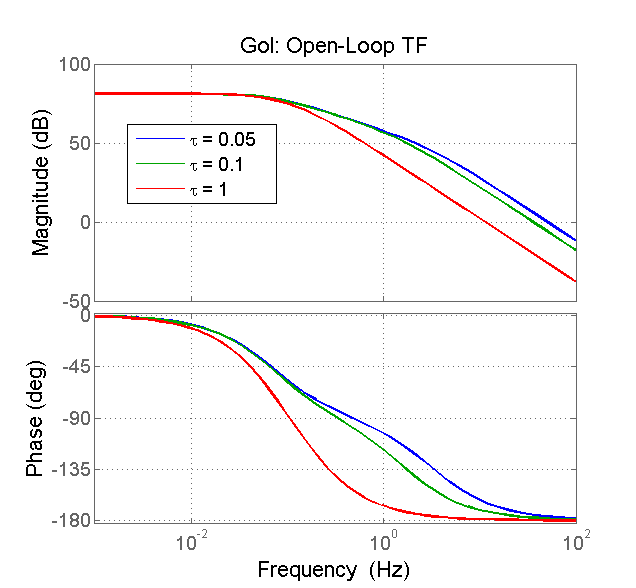
\includegraphics[scale=0.4]{q3_8}
\caption{$G_{OL}$ as $\tau$}
\label{q3_8}
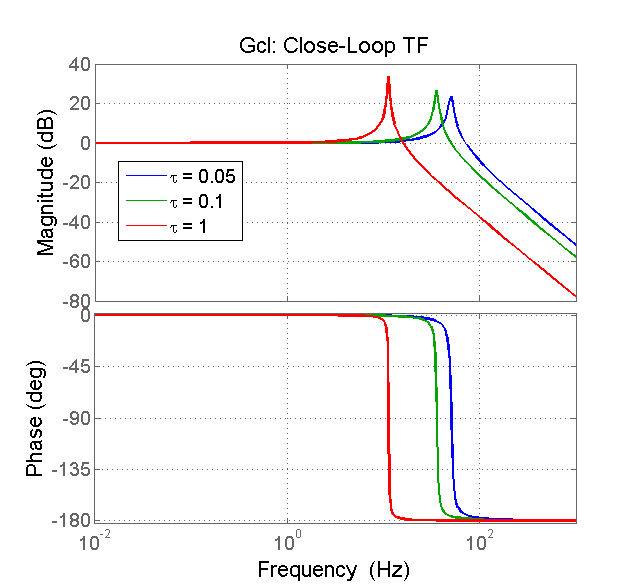
\includegraphics[scale=0.4]{q3_9}
\caption{$G_{CL}$ and $G_{di}$ as $\tau$}
\label{q3_9}
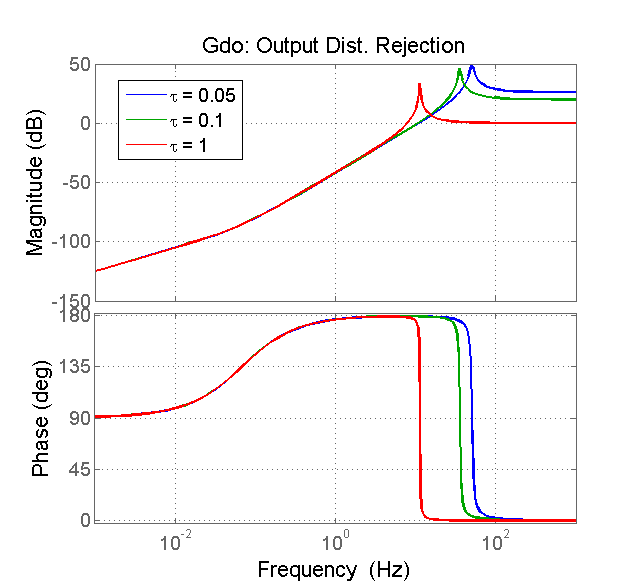
\includegraphics[scale=0.4]{q3_10}
\caption{$G_{do}$ as $\tau$}
\label{q3_10}
\end{center}
\end{figure}
We have already known that $\tau$ is a time constant for the position filter, it does not have direct effect to our controller design. However, a larger $\tau$ will decrease the speed of response of our system and bandwidth, which makes the frequency domain of tracking command signal, output disturbance rejection and sensitivity rejection smaller. As figure \ref{q3_10} shows, increasing $\tau$ will enlarge the frequency domain of sensor noise rejection, input disturbance rejection and and unmodelled dynamic rejection, which is a positive effects of increasing $\tau$.\\

First let us tune the PID controller for velocity control, proportional gain, integral gain and derivative gain are denoted as $K_{VP}$, $K_{VI}$ and $K_{VD}$.

\subsubsection*{d) Keep steady state error below 2\% for a step command of 2$\pi$ radians/sec}
Tuning practices to achieve satisfactory step response:
\begin{itemize}
\item Initialize $\tau$ as 0.05 to begin with.
\item Tune $K_{VP}$ as high as possible because when $K_{VP}$ is increased, the crossover frequency as well as the bandwidth of velocity loop will also increase.
\item If $K_{VP}$ exceeds a certain value, it may affect the system stability or saturate either the actuator or the current driver. Considering this issue, $K_{VP}$ was limited by the maximum peak current (6A) and continuous current (1.92A), respectively. Thus, $K_{VP}$  was tuned to 15, ensuring the commanded voltage less than 1.92 A in steady state.  
\item $K_{VI}$ was not required here since the steady-state error was already less than 2\%. The reason may be because the filter seemed to provide the similar function to the integral gain.
\end{itemize}

\subsubsection*{e) Provide command tracking: Amplitude should remain within 5\% of command up until 5Hz for “command amplitude” of $\pi$/2 radians/sec}
\begin{itemize}
\item 	The tracking error of 5Hz command was up to 10\%, so that we tried to change $\tau$ to achieve better performance.
\item When $\tau$ was 0.7, the error was minimum and fluctuated below 2\%. This modification also generated better track-ability for the step input.
\end{itemize}

\subsubsection*{f) Attenuate a 60Hz noise signal coming in either at the servo-amplifier or the sensor by at least 5 times.}
\begin{itemize}
\item A noise signal with amplitude 0.1 was used to test disturbance rejection. Over 90\% of the input disturbance from the servo amplifier was rejected; while none of the output disturbance, from the sensor was rejected but, even enlarged. Thus increasing τ was required to get better results. 
\item When $\tau$ was changed from 0.7 to 6, the goal of five-times attenuation was achieved. However, we were unable to maintain sinusoidal command tracking due to the lower bandwidth. This was a trade-off which was expected.
\item Considering the limitation of the PI controller, the derivative controller was introduced to add phase lead in our control loop, broadening the bandwidth. By trial and error, finally the three objectives were achieved with the following values of the coefficients:
$$K_{VP} = 25$$
$$K_{VI} = 0$$
$$K_{VD} = 0.2  \ \ (N =100)\footnote{Causality filter for the differentiator}, \text{and}$$
$$ \tau=6.6 $$

\end{itemize}
Setting these values to our PD controller, we will get the following response results.
\begin{table}[htb]
\begin{center}
    \begin{tabular}{|c|c|c|c|c|}
        \hline
        Reference            & Input Amplitude & Output Amplitude & \%Error & Commanded Voltage \\ 
        ~                    & [rad/s]                 & [rad/s]                  & ~       & [Max. V]                   \\ \hline
        (d)Step              & $2\pi$                  & 6.282                    & 0.08\%  & 0.15                       \\ \hline
        (e)Sinusoidal (5Hz)        & $\pi/2$                 & 1.641                    & 4.46\%  & 1.99                       \\ \hline
        (f)Input Disturbance/s & 0.1                     & 0.0072                    & 13 times  & 0.18                       \\ 
        \hline
    \end{tabular}
    \caption{Simulation results for velocity control}
\end{center}
\end{table}

It is really difficult to satisfy all the controlling goals simultaneously by pure PID controller. Since the P gain have been imposed maximum limitations to avoid driver or motor saturation out of maximum continuous winding current (1.92 A in motor windings) and maximum peak current (6 V, in driver op-amp). Meanwhile, there will always exist trade-offs for choosing parameters, that means balancing values that are good for command signal tracking and those that are better for sensor noise or input disturbance rejection should always be an empirical process. The system response results are listed below:

\begin{figure}[H]
\begin{center}
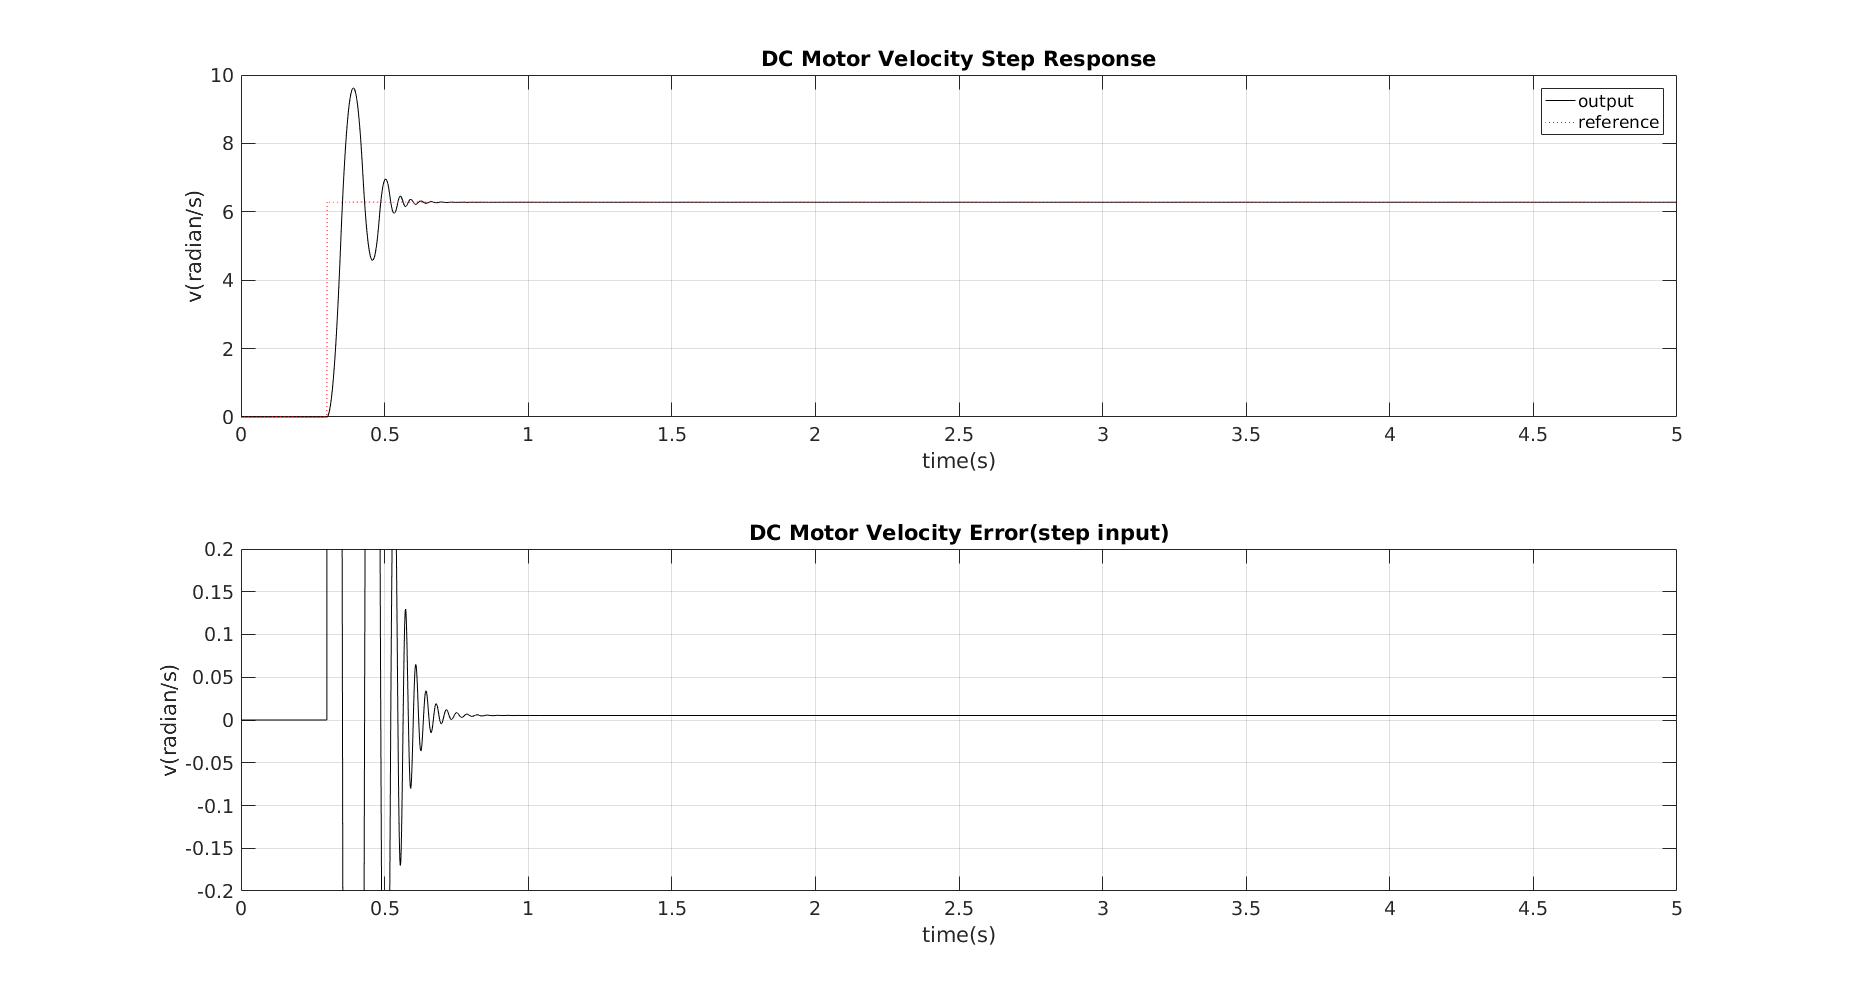
\includegraphics[scale=0.31]{velocity_step.png}
\caption{Step Command of $2\pi$ radians/sec}
\label{q3_12}
\end{center}
\end{figure}
\begin{figure}[H]
\centering
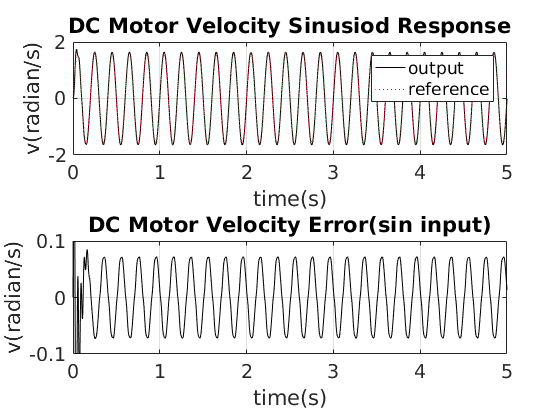
\includegraphics[scale=1]{velocity_sine_5.png}
\caption{5Hz Sinusoidal Command of $\pi/2$ radians/sec}
\label{q3_13}
\end{figure}
\begin{figure}[H]
\centering
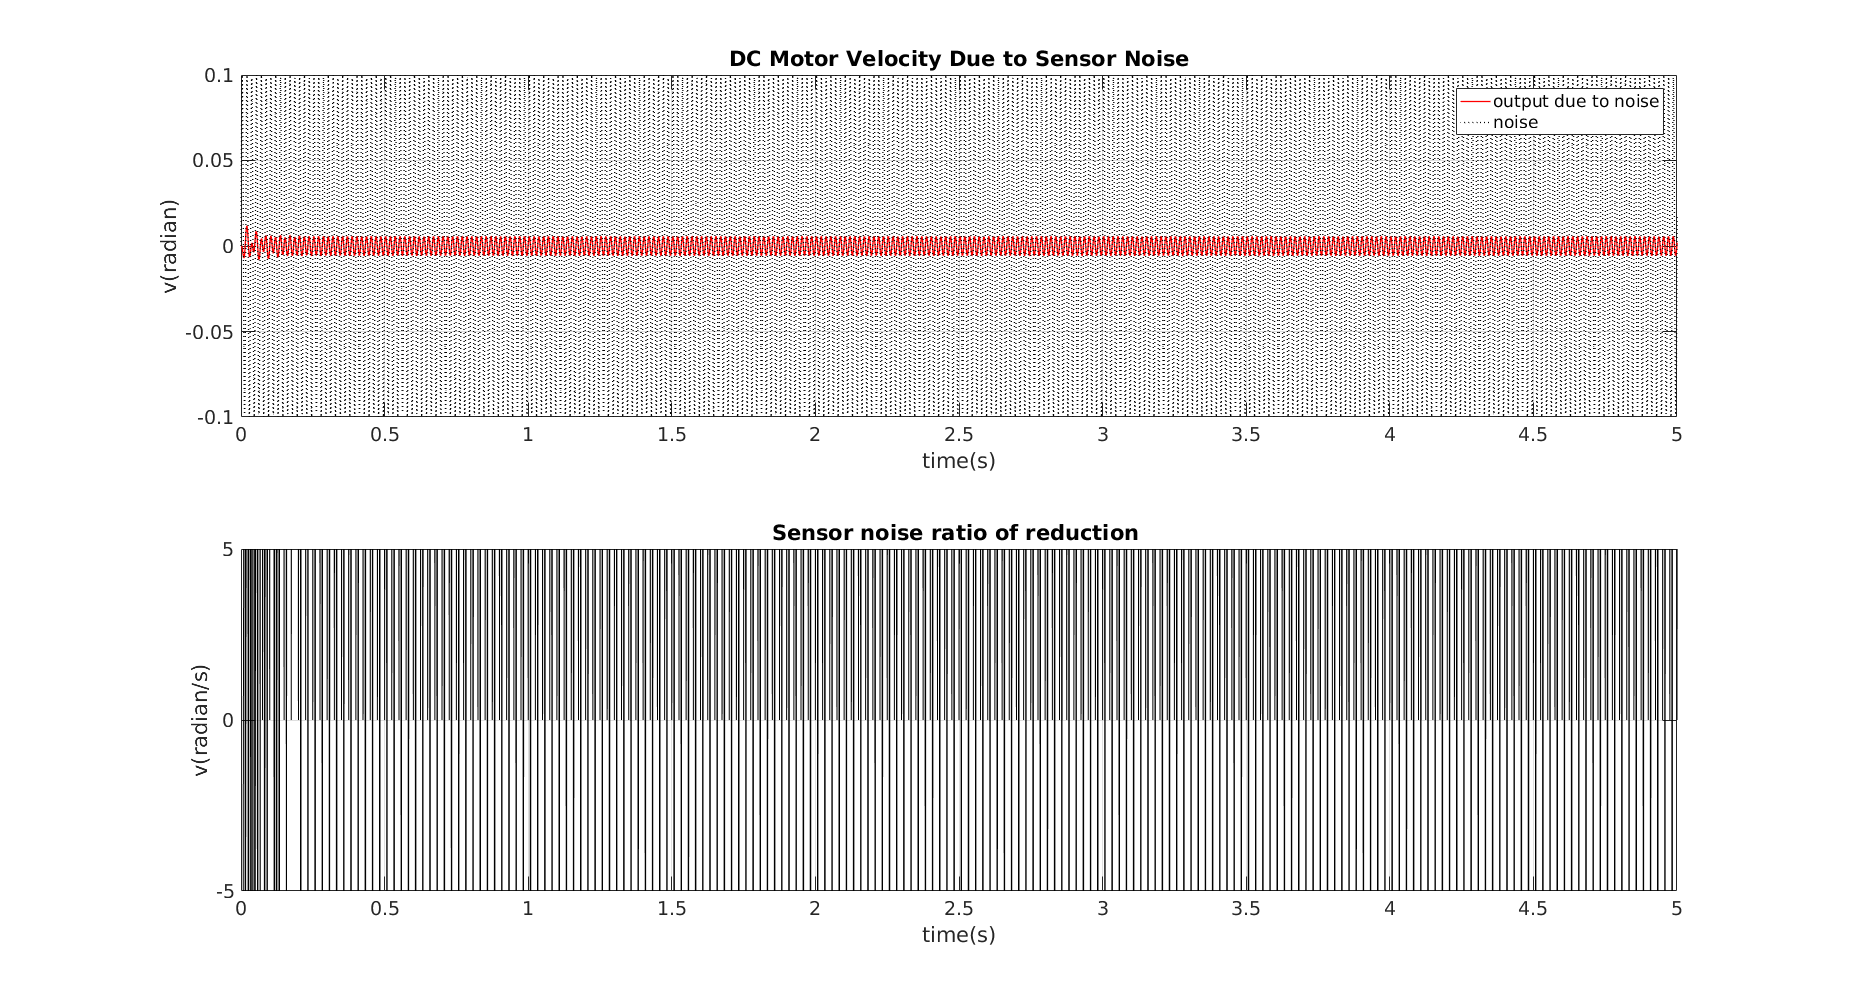
\includegraphics[scale=0.3]{velocity_noise_60.png}
\caption{60Hz Input Disturbance of 0.1 radians/sec}
\label{q3_14}
\end{figure}

\clearpage

For position control system controller design, as shown in figure \ref{q3_16}, there is steady-state error in the tracking function ($G_{CL}$) within the bandwidth (below 0 dB). Furthermore, despite all frequencies are below 0 dB for the transfer function of output disturbance rejection $G_{do}$, there is a peak around 60Hz which should be noticed. Both issues were critical to our objectives of control.

\begin{figure}[H]
\begin{center}
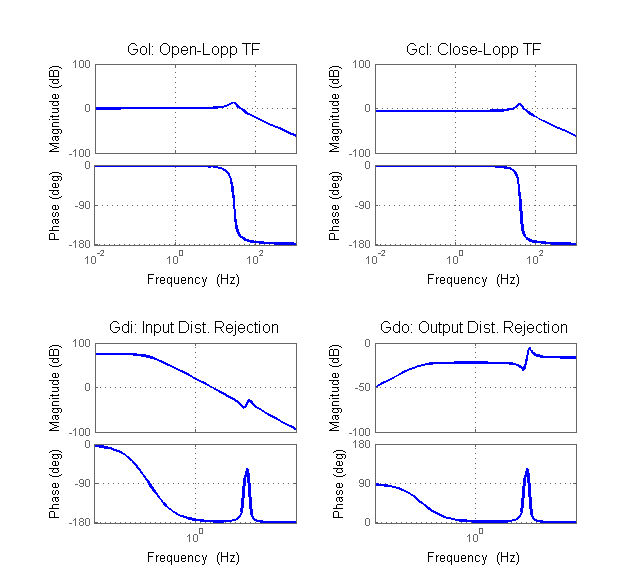
\includegraphics[width = 16 cm]{q3_16}
\caption{Bode Diagrams for the Transfer Functions of Open-Loop ($G_{POL}$), close-loop ($G_{PCL}$), input disturbance rejection ($G_{di}$), and output disturbance rejection ($G_{do}$) }
\label{q3_16}
\end{center}
\end{figure}

We first try to design a PID controller, but we find that if we increase P gain the input voltage to the driver op-amp which will exceed the maximum continuous current, hence we decide to add a feedforward controller. Additionally, in order to decrease the steady state error, we can choose to add a feedforward controller or instead we can choose to tune integral gain in the PID controller. However, increase I gain may effect the stability of our system, so we will set I gain to 0 here and only replace it with a feedforward controller. The parameters for our controller are denoted as: $K_{PP}$, $K_{PD}$ and $K_{VF}$.

\subsubsection*{a) Keep steady state error below 2\% for a step command of $\pi$ or $1$ radians.}
\begin{itemize}
\item Setting $K_{PP}=1$, we see that the error did not fall below the required value. This is because if $K_{PP}$ was increased until the goal was attained, the commanded voltage exceeded the continuous current limit (2A).

\item In order to solve the problem, velocity feedforward control ($K_{VF}$) was introduced to provide better tracking performance without affecting the stability of the closed-loop system.

\item When $K_{VF} = 1$, the tracking error became nearly zero. 
\end{itemize}

\subsubsection*{b) Provide command tracking: Amplitude should remain within 5\% of commanded amplitude of pi radians, up until 5Hz.}
\begin{itemize}
\item With the identical setting, the tracking error of 5Hz command was close to zero as well.    
\end{itemize}


\subsubsection*{c) Attenuate a 60Hz noise signal coming in either at the servo-amplifier or the sensor by at least 10 times.}
\begin{itemize}
\item	A noise signal with amplitude 0.1 was used to test disturbance rejection. For the input disturbance (from servo amplifier), over 90\% was rejected; while none of the output disturbance (from the sensor) was rejected but at times, it was seen to even enlarge. 

\item The above situation was similar to that in the velocity control system, but $\tau$ was already tuned for the velocity loop. Therefore, we needed the derivative controller to improve the quality of disturbance rejection.  

\item Achieving all objectives simultaneously seemed to be impossible due to the limit on the commanded voltage (2A); in particular, the 60Hz noise was hardly  attenuated five times. Thus, we removed the quantizer to get a more favorable system. 

\item By trial and error, finally three objectives were achieved with $K_{PP}=2$, $K_{PD}=0.09 (N)\footnote{Simulinks causality filter}=150$, $K_{VF}=1$, and $\tau = 6.6$. However, the ability of output disturbance rejection was limited with amplitude 0.08. If the noise exceeded this limit, the commanded voltage would go beyond the current limit; that is, more power was required.
\end{itemize} 
\begin{table}[H]
\begin{center}
    \begin{tabular}{|c|c|c|c|c|}
        \hline
        Reference               & Input Amplitude  & Output Amplitude  & \%Error & Commanded Voltage  \\ 
        ~                       & [rad]          & [rad]           & ~       & [Max. V]           \\ \hline
        (a) Step                & $1$              & 0.989             & 0.10\%  & 0.13               \\ \hline
        (b) Sinusoidal (5Hz)          & $\pi$              & 3.144             & 0.16\%  & 0.3                \\ \hline
        (c) Input Disturbance (200 Hz)   & 0.1              & 0.012             & 8.33 times  & 1.55               \\ 
        \hline
    \end{tabular}
\caption{Simulation results for position control}
\end{center}
\end{table}

Position control is based on velocity control, if we have tuned PD controller for velocity control, then we can tune Feedforward/PD controller for position control, the cascaded controller inevitably decrease the accuracy and precision of controller. However, we can still implement this cascaded controller to make sure the closed loop performance satisfy performance specifications in this question. For this problem, we choose to use a feedforward controller which is not an integral controller in PID part, avoiding stability problems at the same time decreasing the steady state error.

\begin{figure}[H]
\begin{center}
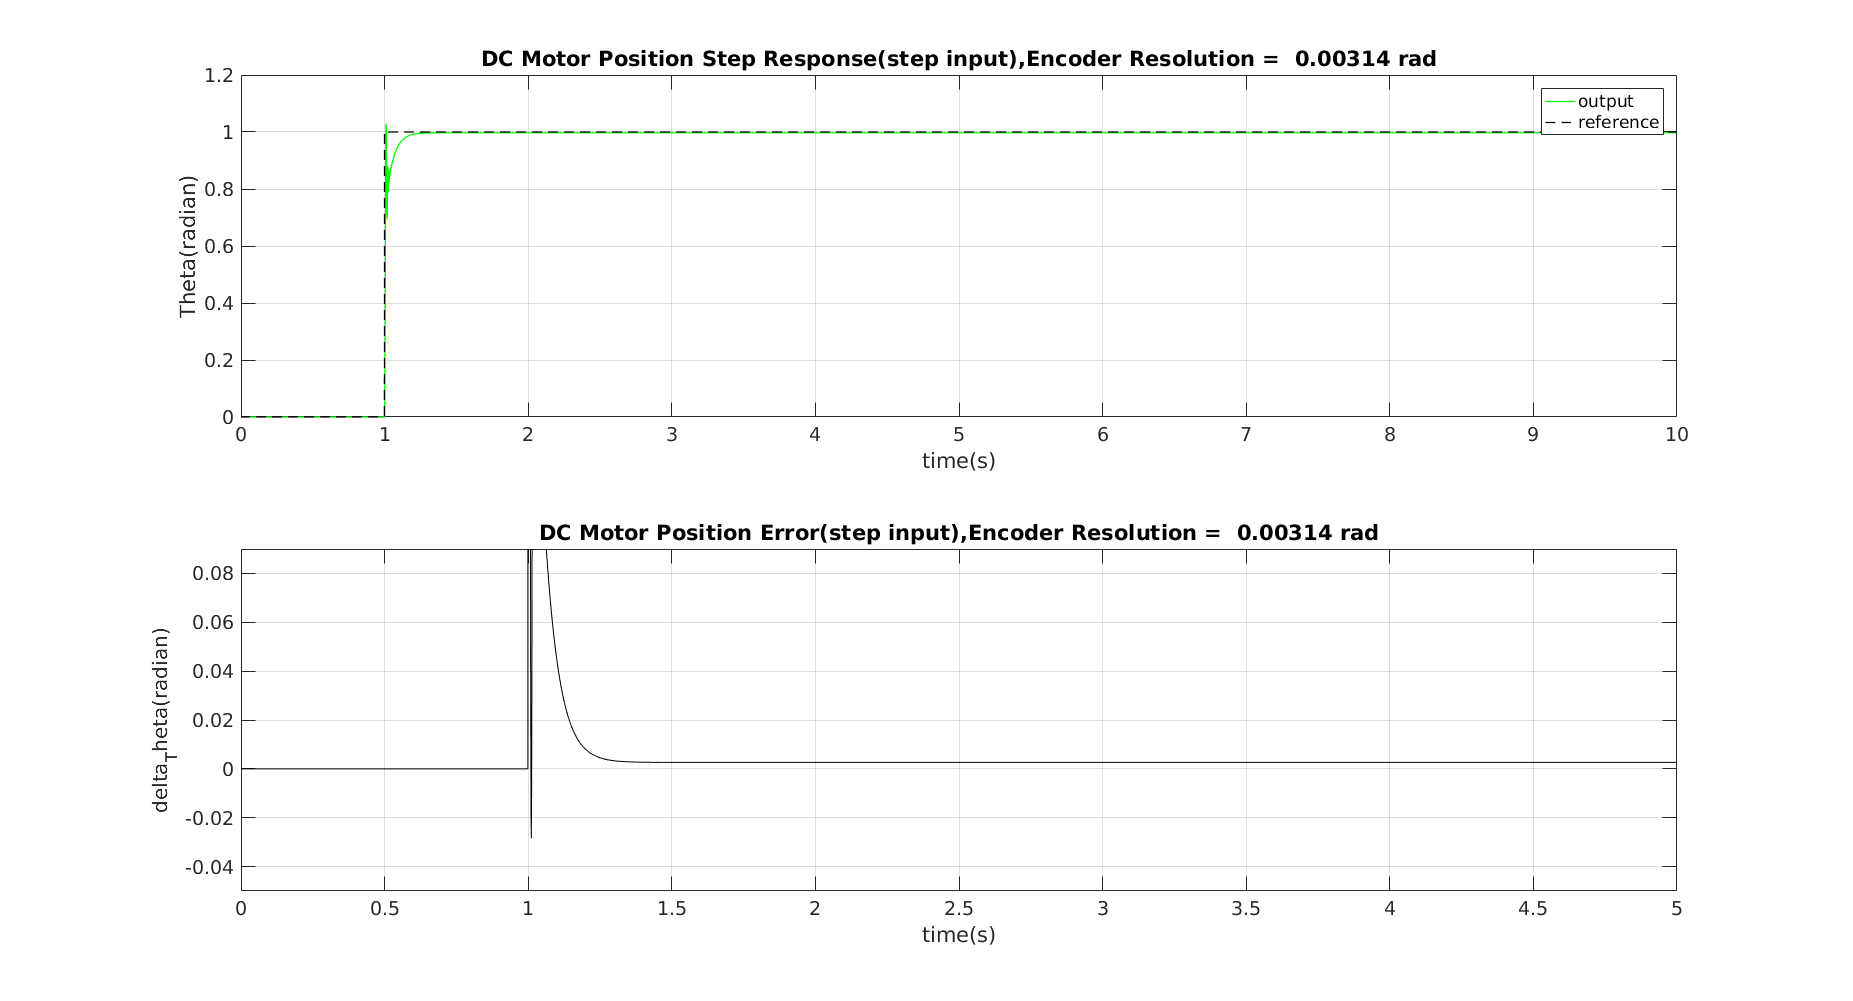
\includegraphics[scale=0.3]{position_step.png}
\caption{Step Command of $1$ radians}
\label{q3_18}
\end{center}
\end{figure}

\begin{figure}[H]
\begin{center}
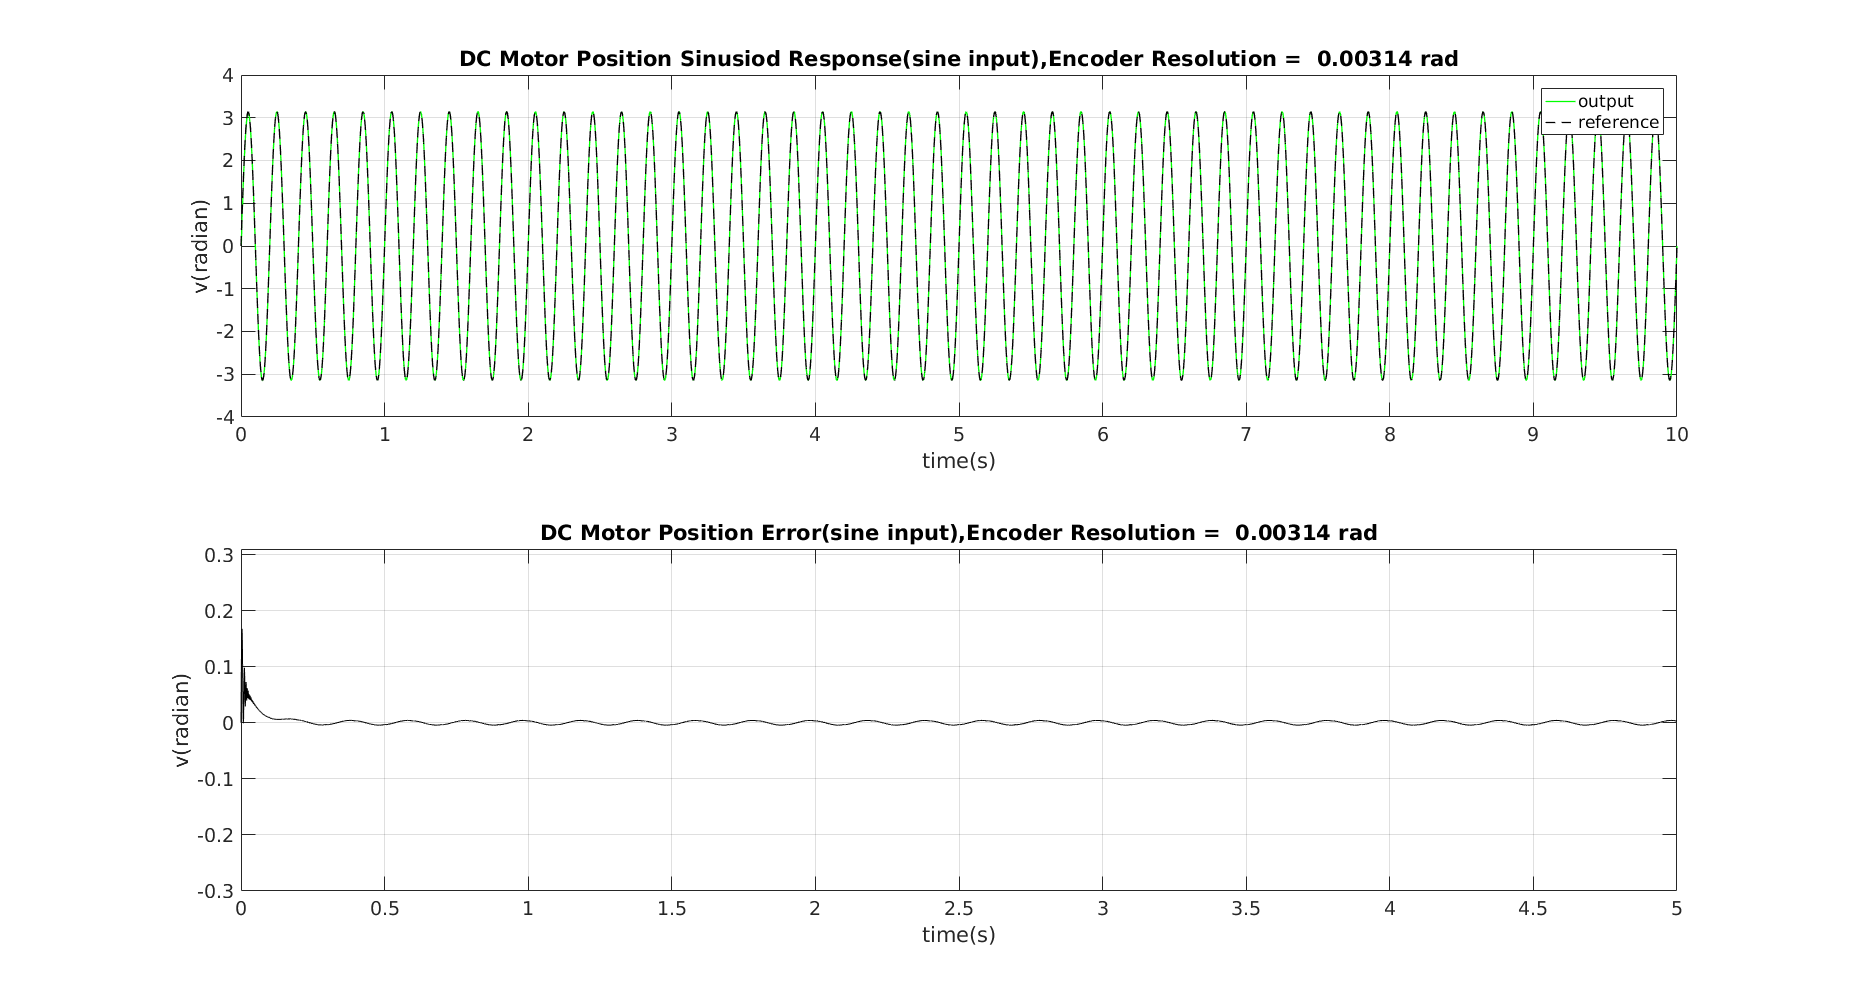
\includegraphics[scale=0.3]{position_sine.png}
\caption{5Hz Sinusoidal Command of $\pi$ radians/sec}
\label{q3_19}
\end{center}
\end{figure}

\begin{figure}[H]
\begin{center}
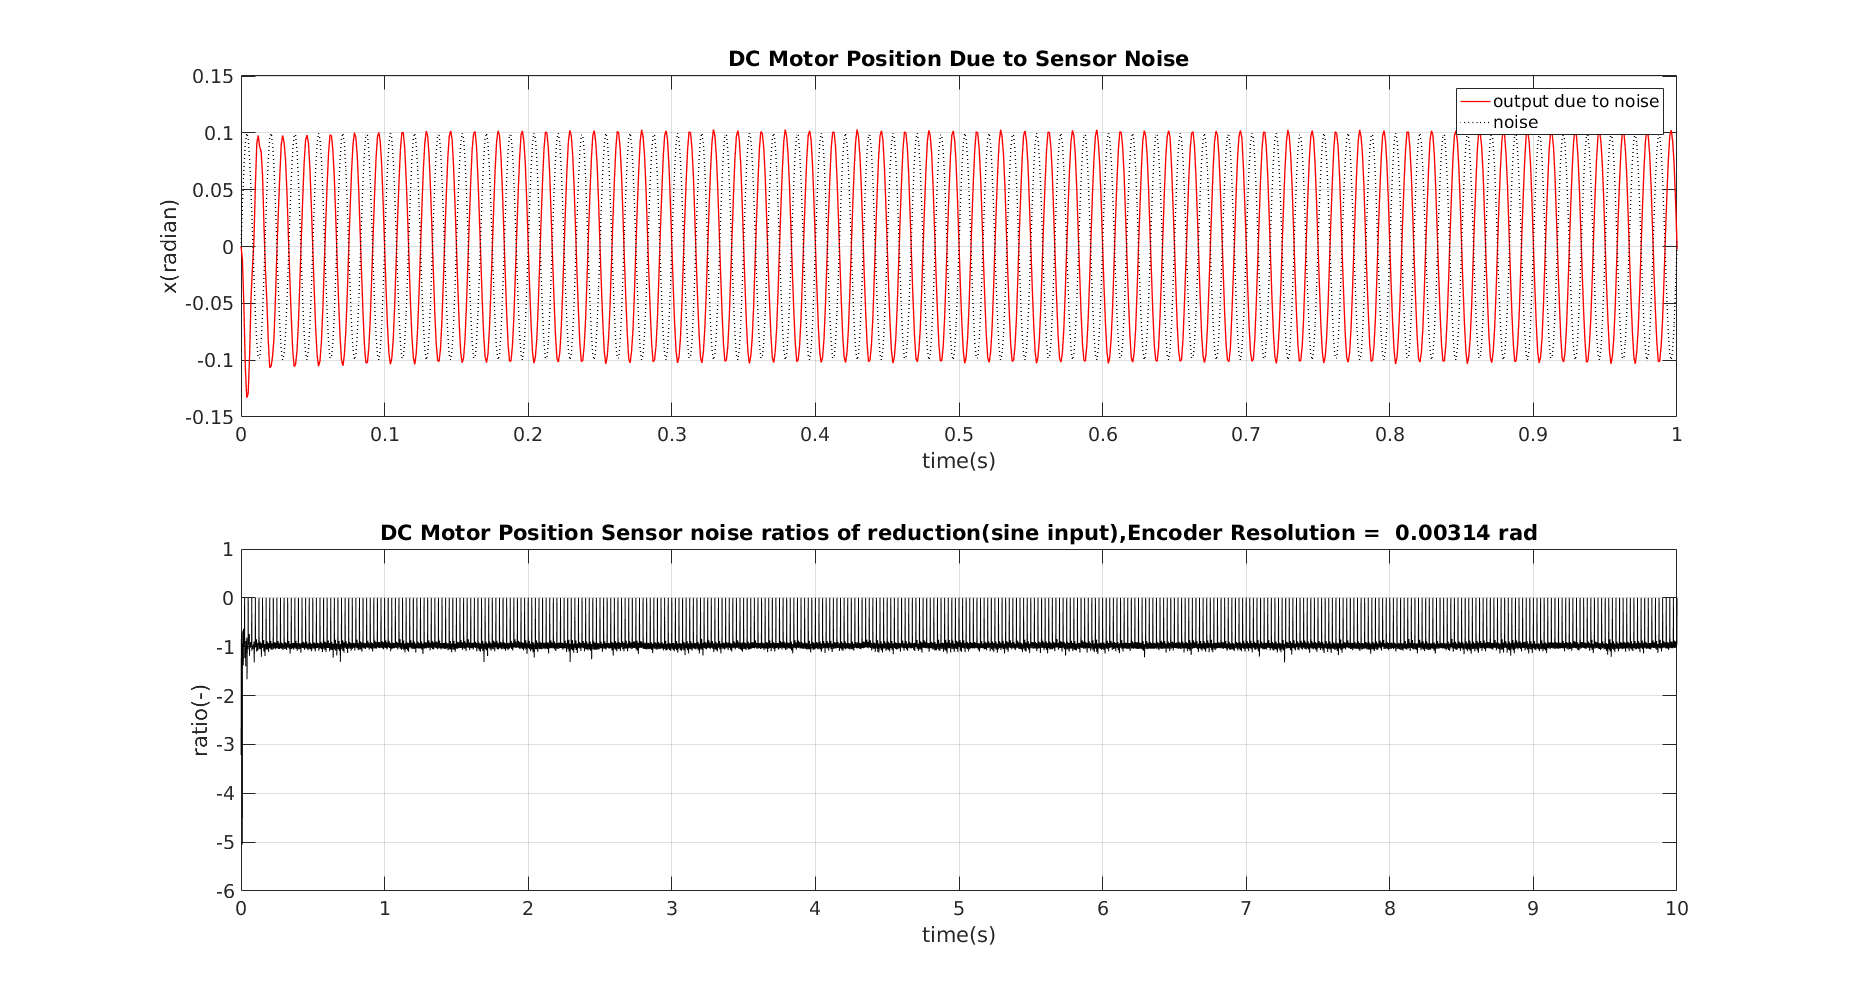
\includegraphics[scale=0.3]{position_noise_60.png}
\caption{60Hz sensor noise of 0.1 radians}
\label{q3_18}
\end{center}
\end{figure}

\begin{figure}[H]
\begin{center}
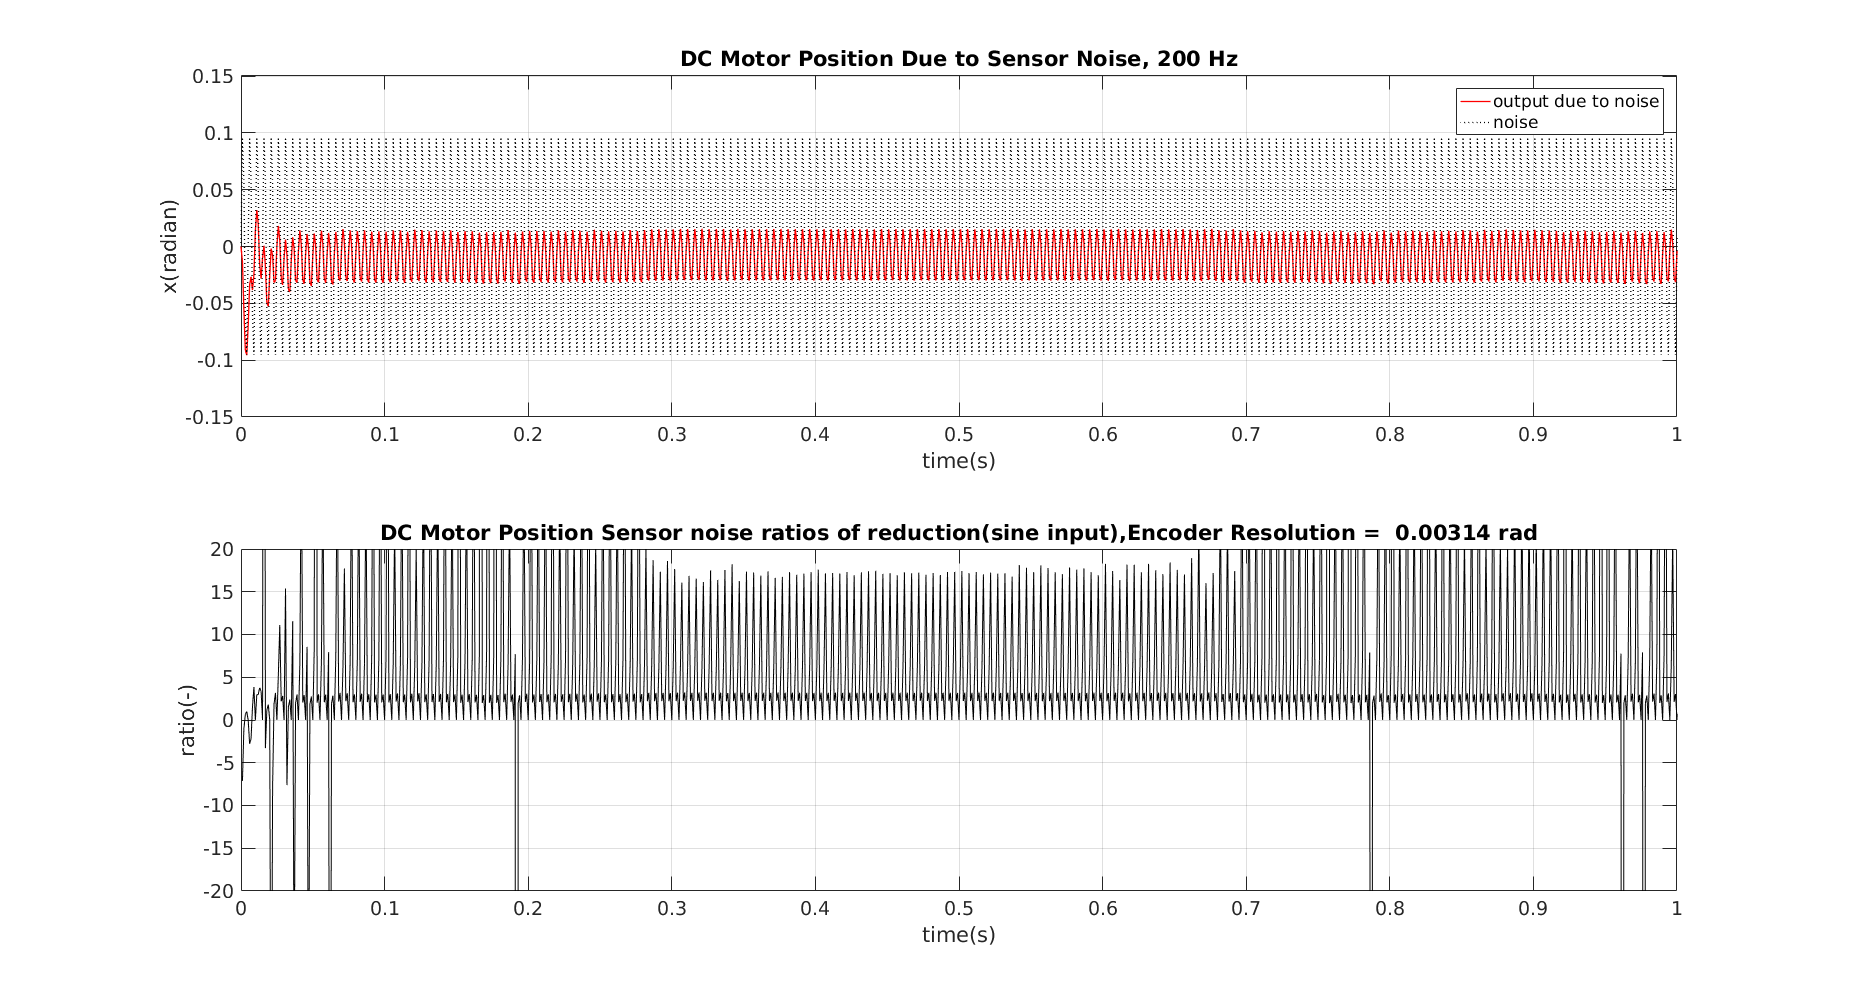
\includegraphics[scale=0.3]{position_noise_200.png}
\caption{200Hz input disturbance of 0.1 radians}
\label{q3_21}
\end{center}
\end{figure}

\clearpage

\section*{Question 4}
\subsection*{(a)}
When we implemented the controller and values from our simulation in part 3, we were unable to achieve stable output in the physical system. Therefore, we kept the same general approach - a velocity controller nested within a position controller with feed forward - but we re-tuned the system with different gain values. Because we have a velocity controller inside of our position controller, we first tuned the velocity control on its own (see section 6). Once it was working, we then implemented it in the inner loop of our position controller and tuned the position control gains. In the end we were not able to meet all of the control goals with one controller. We designed one controller with good step response and noise attenuation, and then modified the gain values to improve the frequency response separately. The results for the step response and noise attenuation are given below.\\


\begin{table}[htb]
\begin{center}
    \begin{tabular}{|c|c|c|c|c|c|}
        \hline
        Gains & P   & I & D   & Feed Forward   & Filter $\tau$   \\ \hline
        Position Loop            & 0.1 & 20  & 0 & 1 & 6.5797    \\ 
        Velocity Loop       & 22.5   & 22.5    & 1.125   & -  & 6.5797  \\ 
       \hline
    \end{tabular}
\end{center}
\caption{Values of position controller with nested velocity controller for step response and noise attenuation}
\label{positionGains}
\end{table}

Figure \ref{PosStepPi} shows the system's response to a position step input of $\pi$ radians, and figure \ref{PosStepError} shows a zoomed in view after it had settled. The peak error here is 0.11\%, which out performs the goal of 2\% error. Additional results for position steps of different magnitudes are included in section 5b.  The error seen here is very similar to the steady state error of 0.10\% predicted in our simulink simulation in response to a step input of $1$ radians.\\

\begin{figure}[H]
\begin{center}
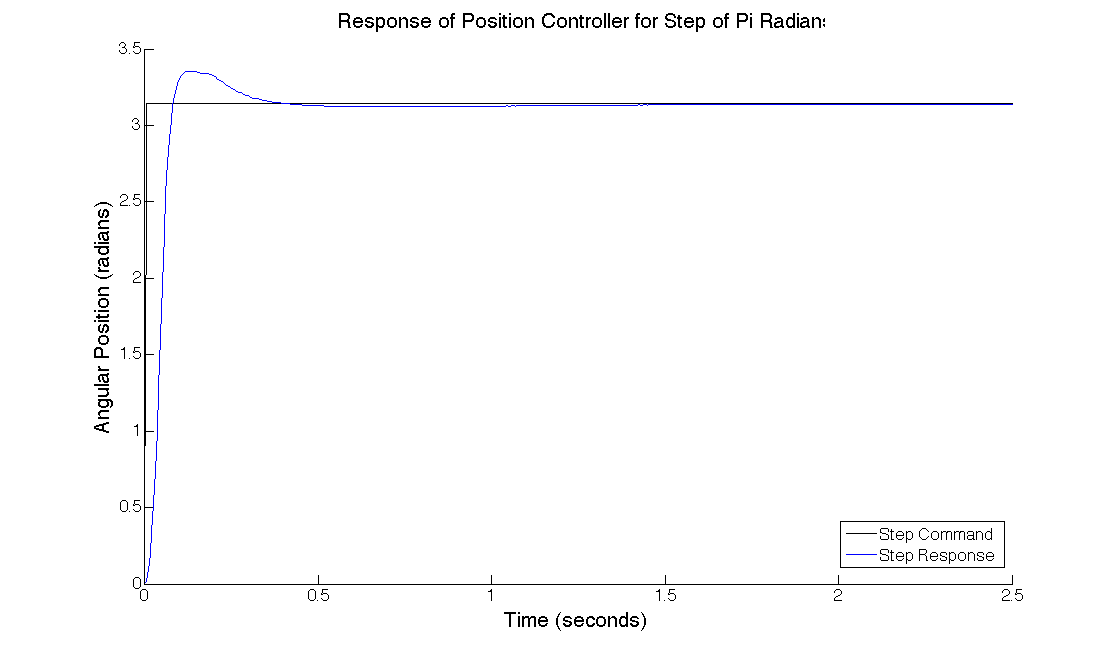
\includegraphics[scale=0.2]{posstep_1pi.png}
\caption{Step response of position controller}
\label{PosStepPi}
\end{center}
\end{figure}

\begin{figure}[H]
\begin{center}
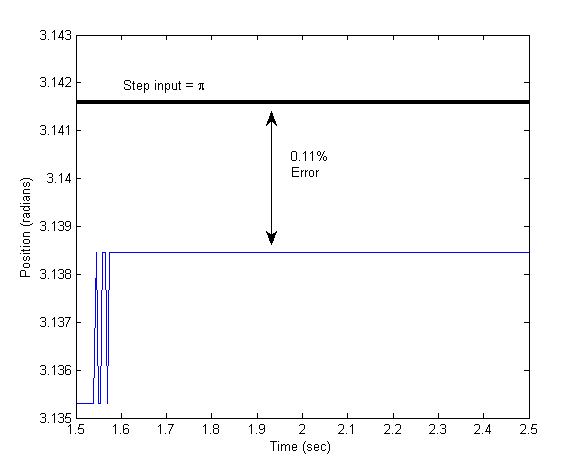
\includegraphics[scale=0.5]{positionStepError.png}
\caption{Steady state error for position step input of $\pi$}
\label{PosStepError}
\end{center}
\end{figure}

Figure \ref{PosNoise} shows the noise attenuation during a step input of $\pi$ radians. To simulate the noise within LabView, we added a 60 Hz sine signal with an amplitude of 1 to the output of the DAQ assistant. Figure \ref{PosNoiseZoom} shows a zoomed in view after the step has taken place. For the step response with no noise, our steady state error was approximately 0.003, and with the noise the highest error is 0.060. Given that we were inputting a noise amplitude of one and the error only increased by 0.057, we have attenuated the noise by approximately 17.54 times. This exceeds the goal of a ten times reduction.\\

\begin{figure}[H]
\begin{center}
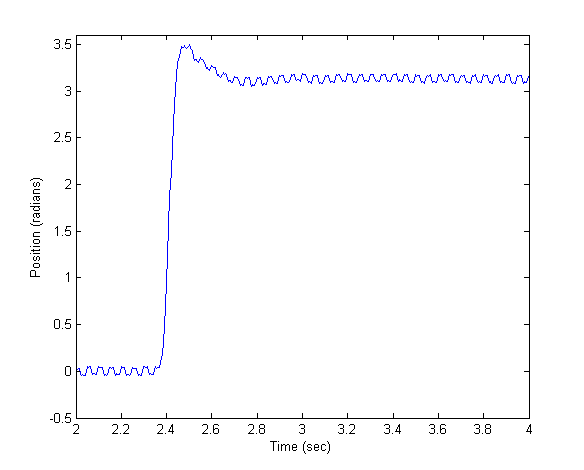
\includegraphics[scale=0.5]{PosNoise.png}
\caption{Step response for input of $\pi$ with a 60 Hz noise signal (amplitude = 1)}
\label{PosNoise}
\end{center}
\end{figure}

\begin{figure}[H]
\begin{center}
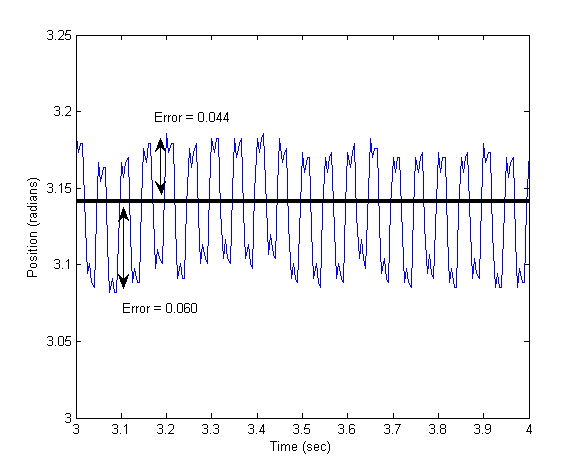
\includegraphics[scale=0.5]{PosNoiseZoom.png}
\caption{Steady state step response for input of $\pi$ with a 60 Hz noise signal (amplitude = 1)}
\label{PosNoiseZoom}
\end{center}
\end{figure}

The position controller we were using for the step response and noise attenuation did not not perform well with sinusoidal inputs forcing us to modify gains while keeping the overall architecture the same. The relevant values are given in the table \ref{positionFreqGains}, and the following figures show the response at various frequencies with an amplitude of $\pi$. Figure \ref{PosFreqError} shows the error as a function of input frequency. During our tests the position output remained stable up to 5 Hz, but the output amplitude error exceeded 5\% just beyond 4 Hz. This does not meet the goal of less than 5\% error up to 5 Hz.  The performance of the real system at 5 Hz with an output magnitude of -2.078 dB performs far worse than our simulated system which maintained a 0 dB magnitude at the same frequency, the Table \ref{q4_atable} shows the simulation results when we try to input a series of sine waves with frequencies from 1 Hz to 5.72 Hz. \\

\begin{table}[H]
\begin{center}
    \begin{tabular}{|c|c|c|c|c|c|}
        \hline
        Gains & P   & I & D   & Feed Forward   & Filter $\tau$   \\ \hline
        Position Loop            & 0 & 20  & 0 & 1 & 6.5797    \\ 
        Velocity Loop       & 3   & 7    & 0.4   & -  & 6.5797  \\ 
       \hline
    \end{tabular}
\end{center}
\caption{Values of position controller with nested velocity controller for frequency response}
\label{positionFreqGains}
\end{table}

\begin{table}[H]
    \begin{tabular}{|c|c|c|c|c|}
        \hline
        Frequency (Hz) & Input Amplitude & Output Amplitude & Magnitude (dB) & \%Error       \\ \hline
        1              & $\pi$           & 3.13845          & -0.008693172   & -0.100033771 \\ 
        2              & $\pi$           & 3.02221          & -0.336504689   & -3.800067888 \\ 
        3              & $\pi$           & 3.079209         & -0.174214105   & -1.985733367 \\ 
        4              & $\pi$           & 3.030152         & -0.313709167   & -3.547266176 \\ 
        5              & $\pi$           & 2.473084         & -2.078220099   & -21.27929134 \\ 
        5.27           & $\pi$           & 2.181877         & -3.166392169   & -30.54869805 \\
        \hline
    \end{tabular}
    \caption{Position control data.}
    \label{q4_atable}
\end{table}

To determine the closed-loop bandwidth of the system, we slowly increased the frequency of the input signal until the output amplitude just crossed -3 dB (for a input of $\pi$ this corresponded to an output of 2.22). We found that the bandwidth of our position control system was 5.27 Hz, as shown in figure \ref{PosBandwidth}.

\begin{figure}[H]
\begin{center}
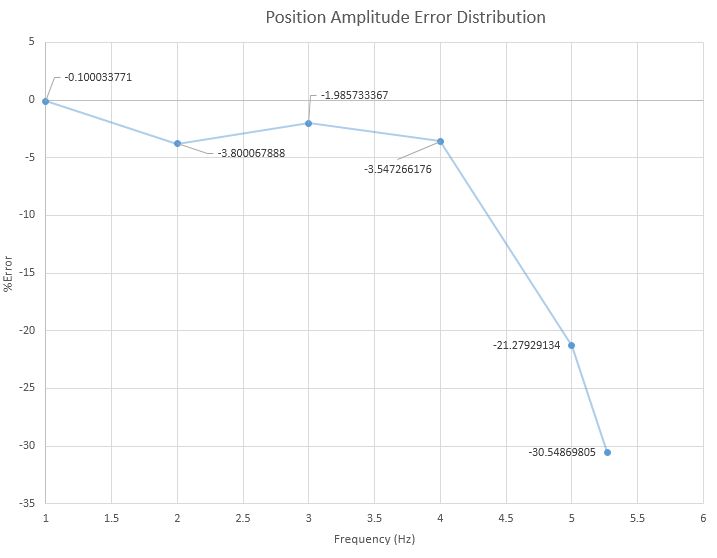
\includegraphics[scale=0.5]{PositionControl_Error.png}
\caption{Position error vs. frequency for an input amplitude of $\pi$ radians}
\label{PosFreqError}
\end{center}
\end{figure}

\begin{figure}[H]
\begin{center}
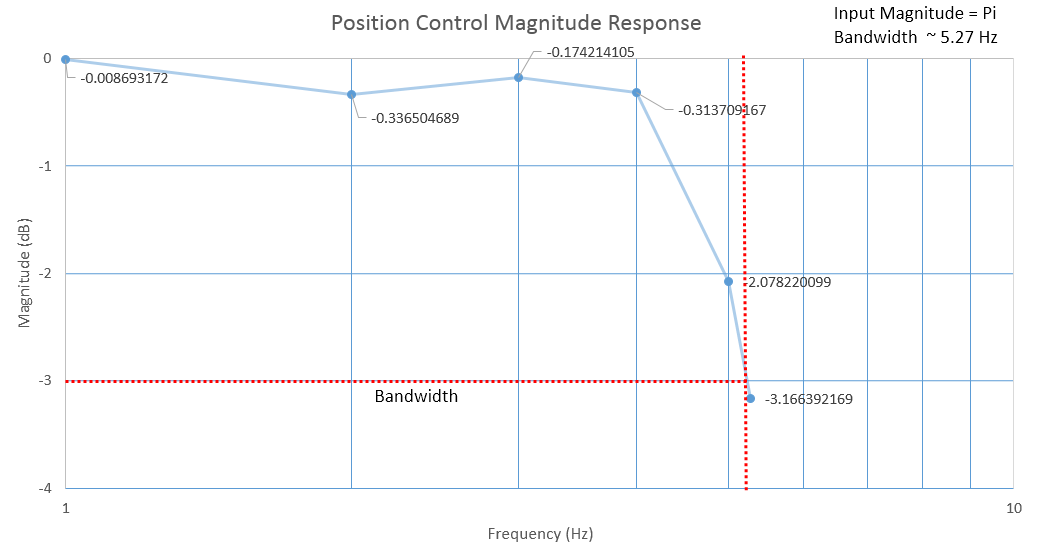
\includegraphics[scale=0.46]{PositionControl_Magnitude.png}
\caption{Output magnitude vs. frequency used to determine bandwidth of position controller}
\label{PosBandwidth}
\end{center}
\end{figure}

Even though we included many nonlinear factors in our simulation, we still faced difficulties meeting all of the performance specifications, particularly trying to do so with just one controller. In general, we found that when we adjusted gains to meet the step requirement, the frequency response usually got worse, and vice-versa. It's possible that some of the values used in our simulation are incorrect (even after testing and regression), or that there are other factors we did not account for, such as the dynamics of the servo-amp. In the end we were able to meet the steady state error for step input and noise attenuation requirements, and were very close to the frequency response requirement.\\

\clearpage

\section*{Question 5}
\subsection*{(a)}
We model Coulomb friction in our Simulink models using a quasi-linear function, Coulomb friction will include dry friction (static friction) and kinetic friction. It is generated mainly due to the relative movement between bearings and rotor inside our DC motor. Meanwhile, there also exists Coulomb friction between brushes and commutator.\\

We have put forward system identification methods for Coulomb friction estimation, here we just list another method to measure the Coulomb friction, first we will input a initial voltage to our system and gradually increase it, in our specific system, we just set a $\tfrac{1}{1}$ relationship between input voltage and driver output current. When our motor starts to rotate, we record the instant voltage and multiply it by a torque constant given in datasheet, we will get the Coulomb friction torque. For kinetic friction, we just conduct a system identification by applying a constant voltage to the system, the motor would come to a steady-state velocity. Since the damping ratio $B$ is given in datasheet, we can calculate the instant motor torque by ($K_{t} \cdot V_{cmd}$), which is used to subtract the torque from damping ($B\cdot\omega$).\\

Friction was included in our Simulink model from the beginning of our modeling, as presented in part 3. In part 3, we also simulate our theoretical system in Simulink incorporated with a Coulomb friction module, based on that we just design a more conservative controller in section 3. By analyzing the simulation results in section 3 and the actual simulation results from Labview, we found there exists large discrepancy between them, we think reasons for that may come from several aspects. First, parameters set to our Simulink model are from datasheet which may be greatly different from the actual values we got in system identification, which make the results quite different from the actual ones. Secondly, we use two sets of PID controller gains separately in the Simulink model and the actual Labview model, which is reasonable to explain why we have different response performance in real and theoretical model respectively. \\

\subsection*{(b)}
For saturation part, we can see a direct effect to the stability of our system.  When our system get saturated, the control signals passed by driver circuits is limited and the actual derivative of signal error can not be feedback to the actuator, meaning that our dynamic system can not respond in real time to our control signal, the rise time of our system will be dependent on values of control signal and stability will also depend on the control signal.  The loss of stability that we see is an effect of integral wind up.  Because the system takes longer to respond, our integral term has a longer period of time to accumulate error, which then has to be canceled out with positive error, leading to large overshoots and long settling times.  In extreme cases this can drive the system to instability.  The effects of saturation on integrator wind up can be compensated for by limiting the maximum and minimum values that the integrator can accumulate.  Another method is to model the saturation effect and use this model to alter the input to the integrator such that when the driver becomes saturated, the integrator no longer receives input. \\

As can be seen in figure \ref{q5_b0} our model also exhibits the same large rise time that we would expect for extremely large input signals.  For an input of $\pi \times 10^{5}$ we see a rise time of roughly, 18 seconds, or 260 times larger than the rise time for a step of $\pi$.  If there was no saturation effect, we would expect to see the exact same rise time.   While our physical system appears to be going unstable for large step magnitudes, the simulation refused to become unstable even for enormous step sizes.   

Our experimental system exhibits distortion due to changes in step size immediately  because our aggressive feed forwards design was already using the all of the available command voltage.
\begin{table}[htb]
\begin{center}
    \begin{tabular}{|c|c|c|c|c|c|}
        \hline
        Step Input Amplitude (Radians) & $1\pi$   & $1.5 \pi$ & $2\pi$   & $3\pi$   & $4\pi$   \\ \hline
        Rise Time (seconds)            & 0.0700002 & 0.0800000   & 0.0850000 & 0.110000 & 0.125    \\ 
        Settling Time (seconds)        & 0.290000   & 0.320000    & 0.28000   & 0.54500  & 1.45500  \\ 
        Percent Overshoot (\%)          & 6.79997   & 16.8000     & 31.8500   & 65.0331  & 91.0003  \\ 
        Steady State Error (\%)         & 0.100034  & 0.594022    & 0.150008  & 0.13335  & 0.399713 \\
        \hline
    \end{tabular}
\end{center}
\caption{Step Response for a variety of input positions.  Where rise time is defined as reaching 90\% of the final value while settling time is the time after which the function remains within 2\% of its final value}
\label{q5_b6}
\end{table}

\begin{figure}[H]
\begin{center}
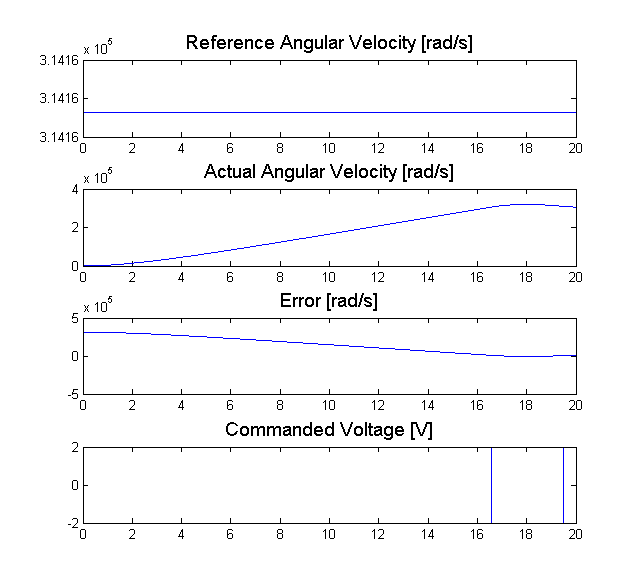
\includegraphics[width = 10cm, height = 8cm]{q5b.png}
\caption{Tracking Ability for Extremely Large amplitude of step command}
\label{q5_b0}
\end{center}
\end{figure}
%^Alex's stuff
\begin{figure}[H]
\begin{center}
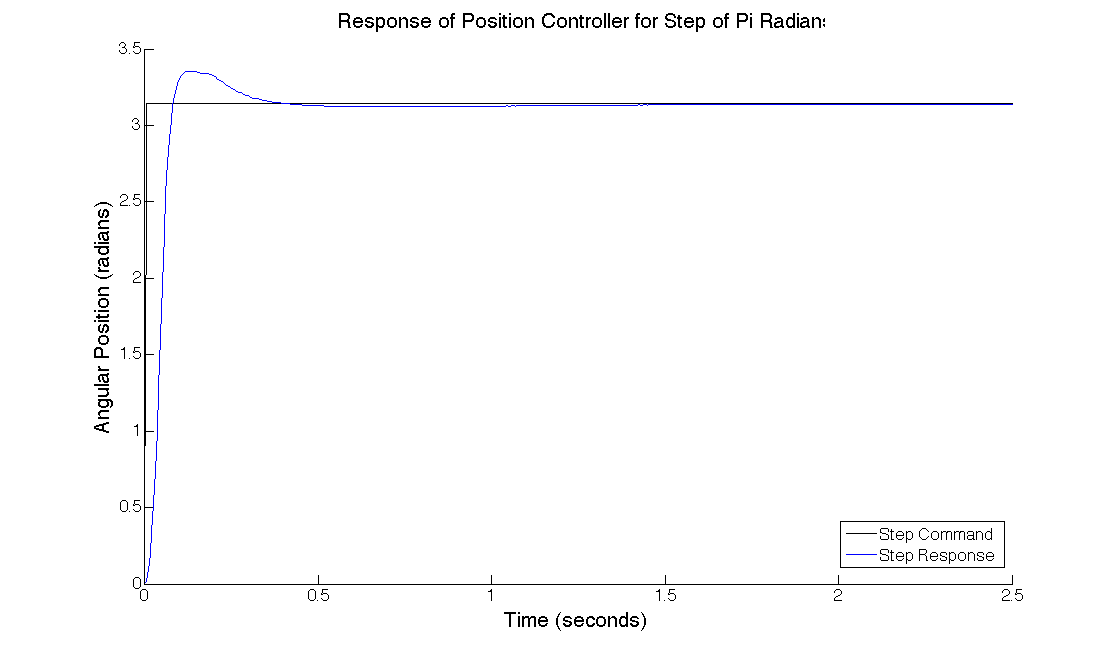
\includegraphics[width = 10cm, height = 5cm]{posstep_1pi.png}
\caption{Step response of position controller}
\label{q5_b1}
\end{center}
\end{figure}

\begin{figure}[H]
\begin{center}
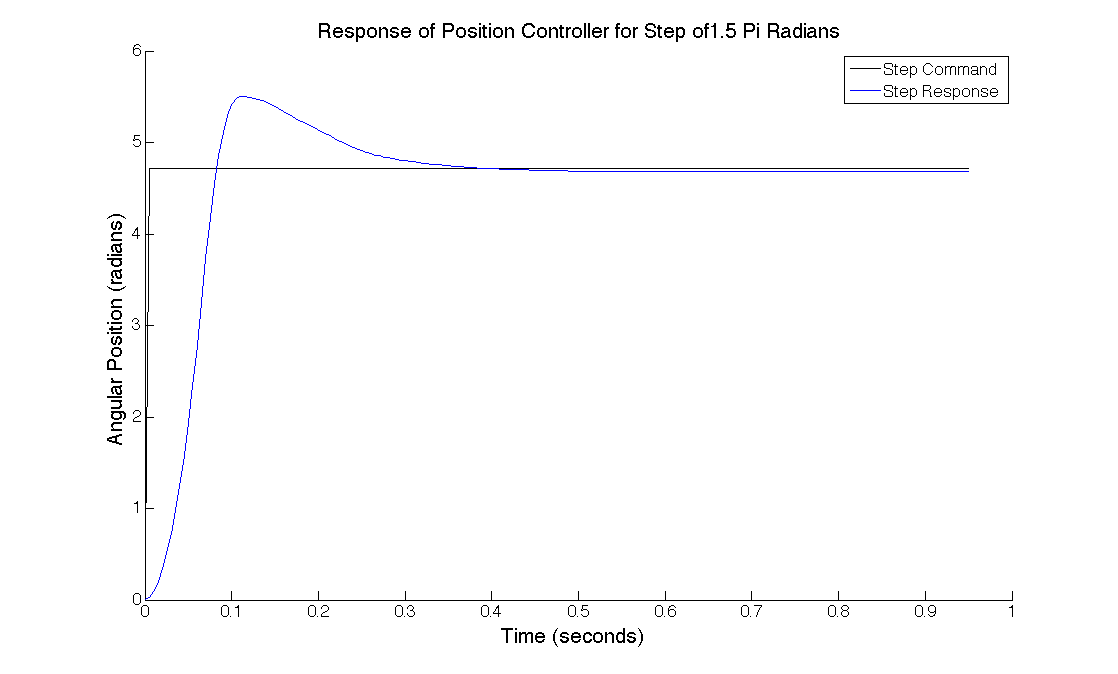
\includegraphics[width = 10cm, height = 5cm]{posstep_15pi.png}
\caption{Step response of position controller}
\label{q5_b2}
\end{center}
\end{figure}

\begin{figure}[H]
\begin{center}
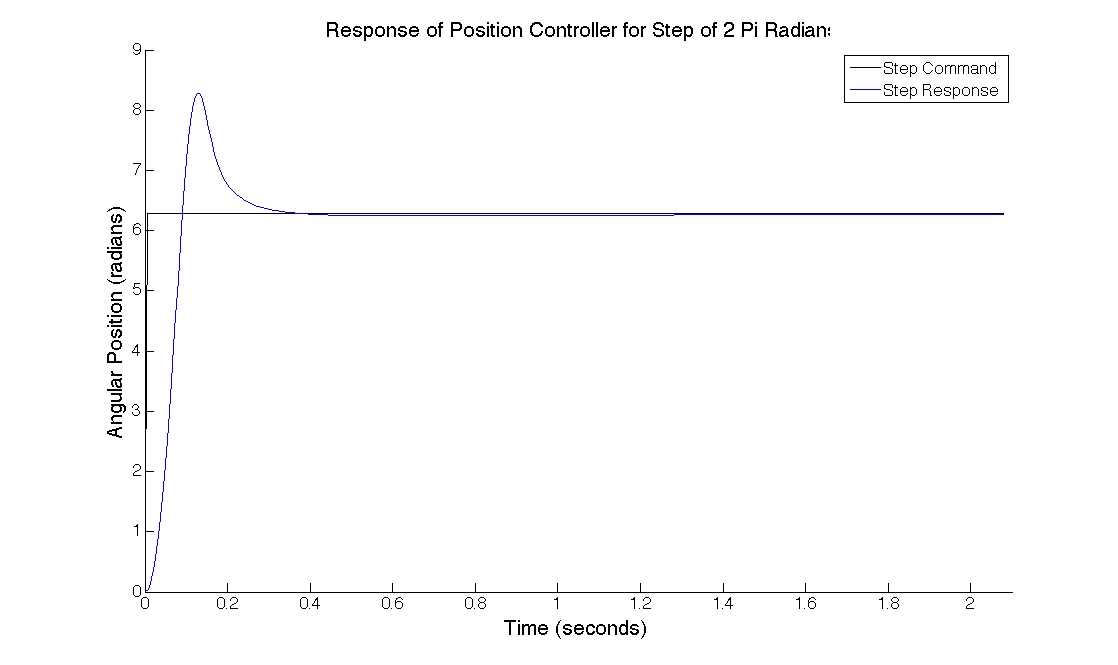
\includegraphics[width = 10cm, height = 5cm]{posstep_2pi.png}
\caption{Step response of position controller}
\label{q5_b3}
\end{center}
\end{figure}

\begin{figure}[H]
\begin{center}
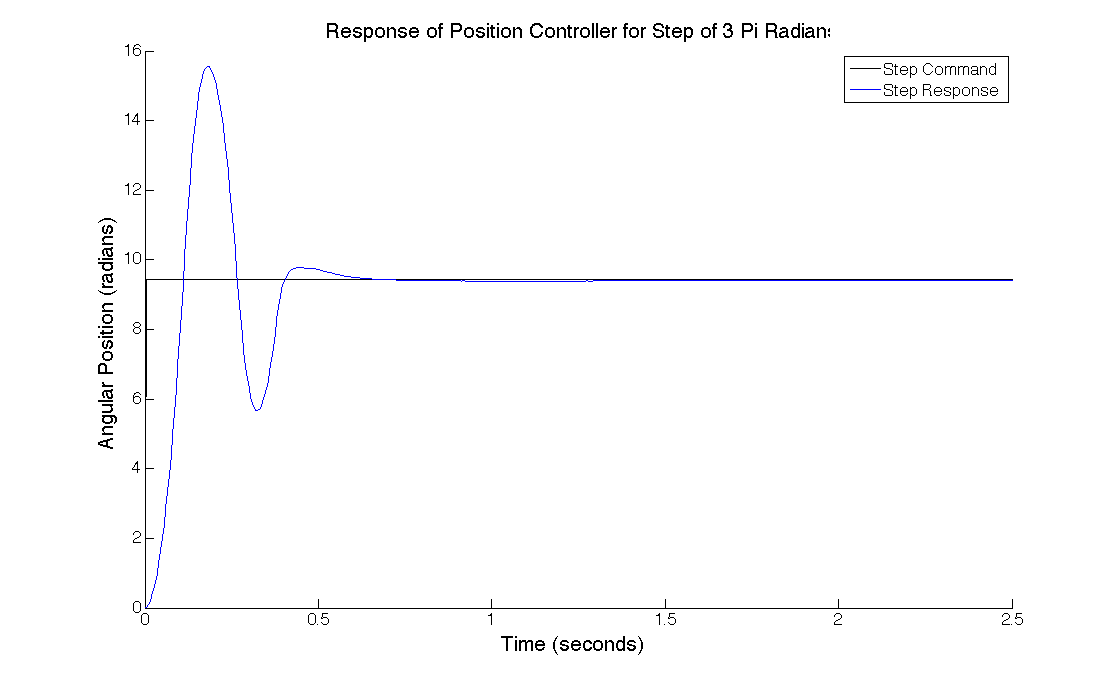
\includegraphics[width = 10cm, height = 5cm]{posstep_3pi.png}
\caption{Step response of position controller}
\label{q5_b4}
\end{center}
\end{figure}

\begin{figure}[H]
\begin{center}
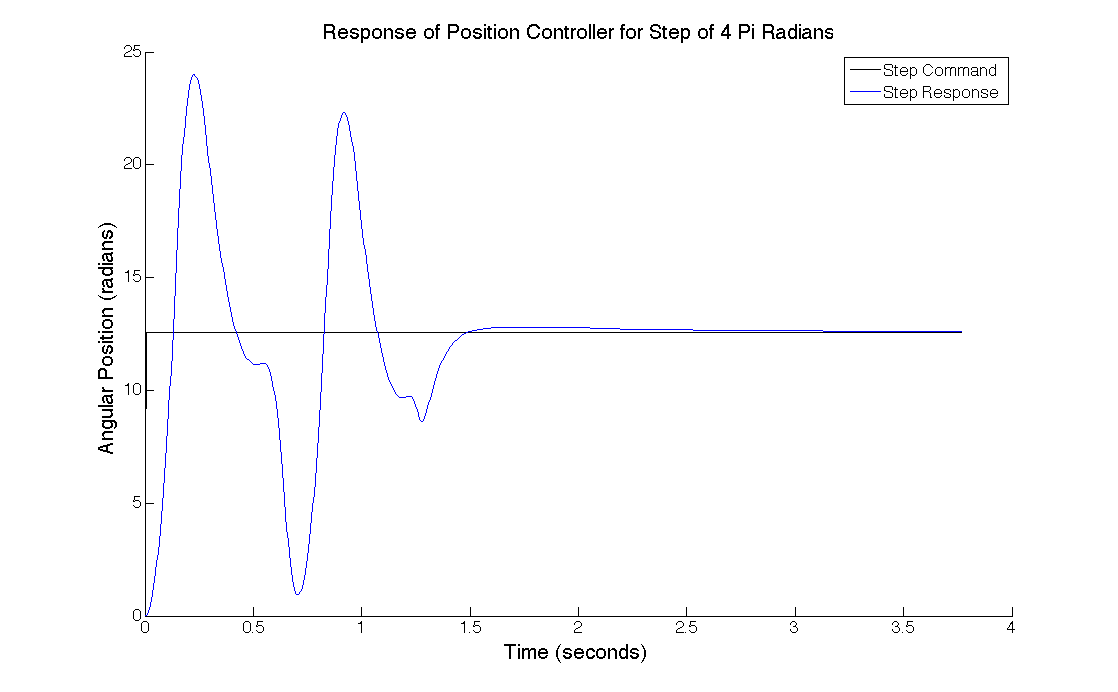
\includegraphics[width = 10cm, height = 5cm]{posstep_4pi.png}
\caption{Step response of position controller}
\label{q5_b5}
\end{center}
\end{figure}

\subsection*{(c)}
The real behavior of the optical encoder was already modeled as the quantizer with an interval $2\pi/2000$ in our model. The higher resolution of the sensor, the closer the system is to a  linear unity gain block, providing less measured error. The tracking error of sinusoidal input exceeded 5\% as the resolution reached 75 step/rev, while the error of step input went beyond 2\% when the resolution neared 325 steps/rev. \\

Most parasitic effects have been considered for our model. For quantization, we find it causes significant trouble in our position control. In feedback control systems, the sum of loop sensitivity  and complementary sensitivity is one. Since the sensed error which resulted from quantization is based on the complementary sensitivity, more power is required to achieve the same closed-loop response; otherwise, the tracking error cannot be lowered in a desired manner. \\

The effects of quantization on velocity estimation cannot be overstated.  Without a proper model of the system velocity estimation requires some sort of filtering to average over previous time steps.  But this introduces a time delay in the velocity estimation and can even cause it to miss quick transients entirely.  

\begin{figure}[H]
\begin{center}
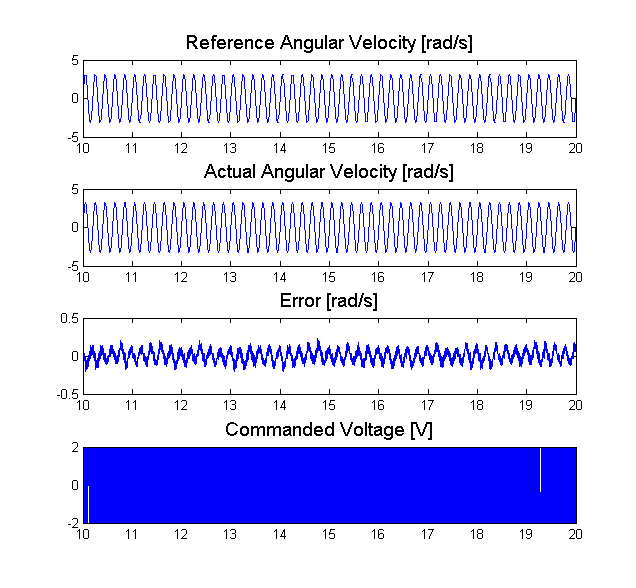
\includegraphics[width = 10cm, height = 6cm]{q5c_sine_75.png}
\caption{Sinusoidal Tracking Error $> 5\%$ when Resolution = 75 steps/rev}
\label{q5_c1}
\end{center}
\end{figure}

\begin{figure}[H]
\begin{center}
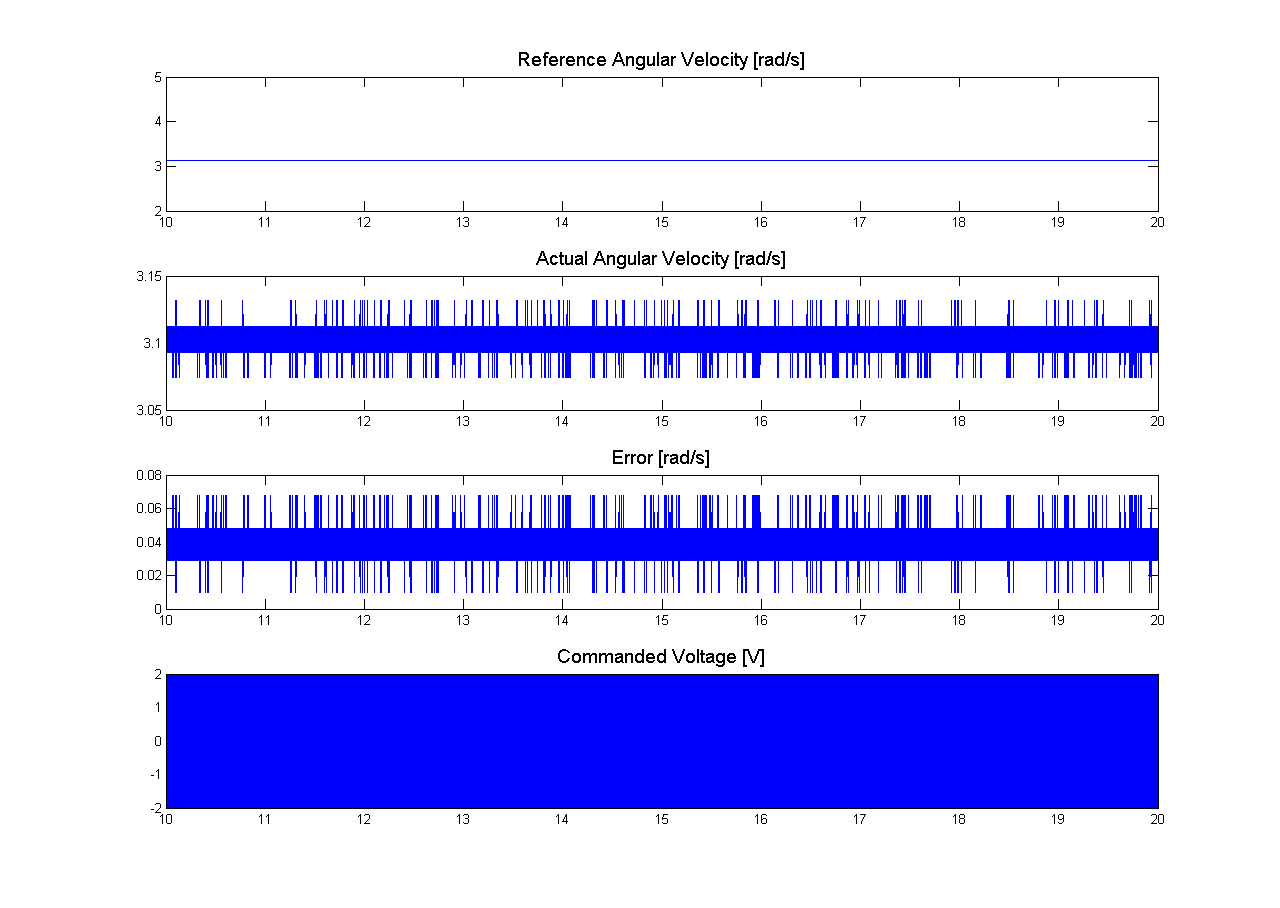
\includegraphics[width = 10cm, height = 6cm]{q5c_step_325.png}
\caption{Step Tracking Error $> 2\%$ when Resolution = 325 steps/rev}
\label{q5_c2}
\end{center}
\end{figure}

\section*{Question 6}
\subsubsection*{Ideal result for step input}
%%%%%%%%%%%%%%%理想的 step 结果
As was discussed in question 4 and 5, work on the velocity controller for the real system was performed before the position controller. In the single position control, we set the three parameters in velocity control $K_p=1$, $K_I=1$, $K_D=0$. Now for velocity control itself, we did face some challenge that the gains we used in the simulation were not able to experimentally stabilize the system with the performance we wanted. Therefor, we create a new PID controller in experiment for velocity control that could meet the step and noise requirements. The new controller in Simulink is shown in Figure. We generate a set of new gain values to improve the frequency response separately. The results for the step response and noise attenuation are given below.\\
\begin{table}[htb]
\begin{center}
    \begin{tabular}{|c|c|c|c|c|}
    \hline
        Gains & P   & I & D     & Filter $\tau$   \\ \hline
        Velocity Controller  & 1.5 & 2.5 & 0.05 & 6.6 \\
    \hline
    \end{tabular}
\end{center}
\caption{Values of velocity controller for step response and noise attenuation}
\label{velocityGains_step_theory}
\end{table}\\

\begin{figure}[htb]
\begin{center}
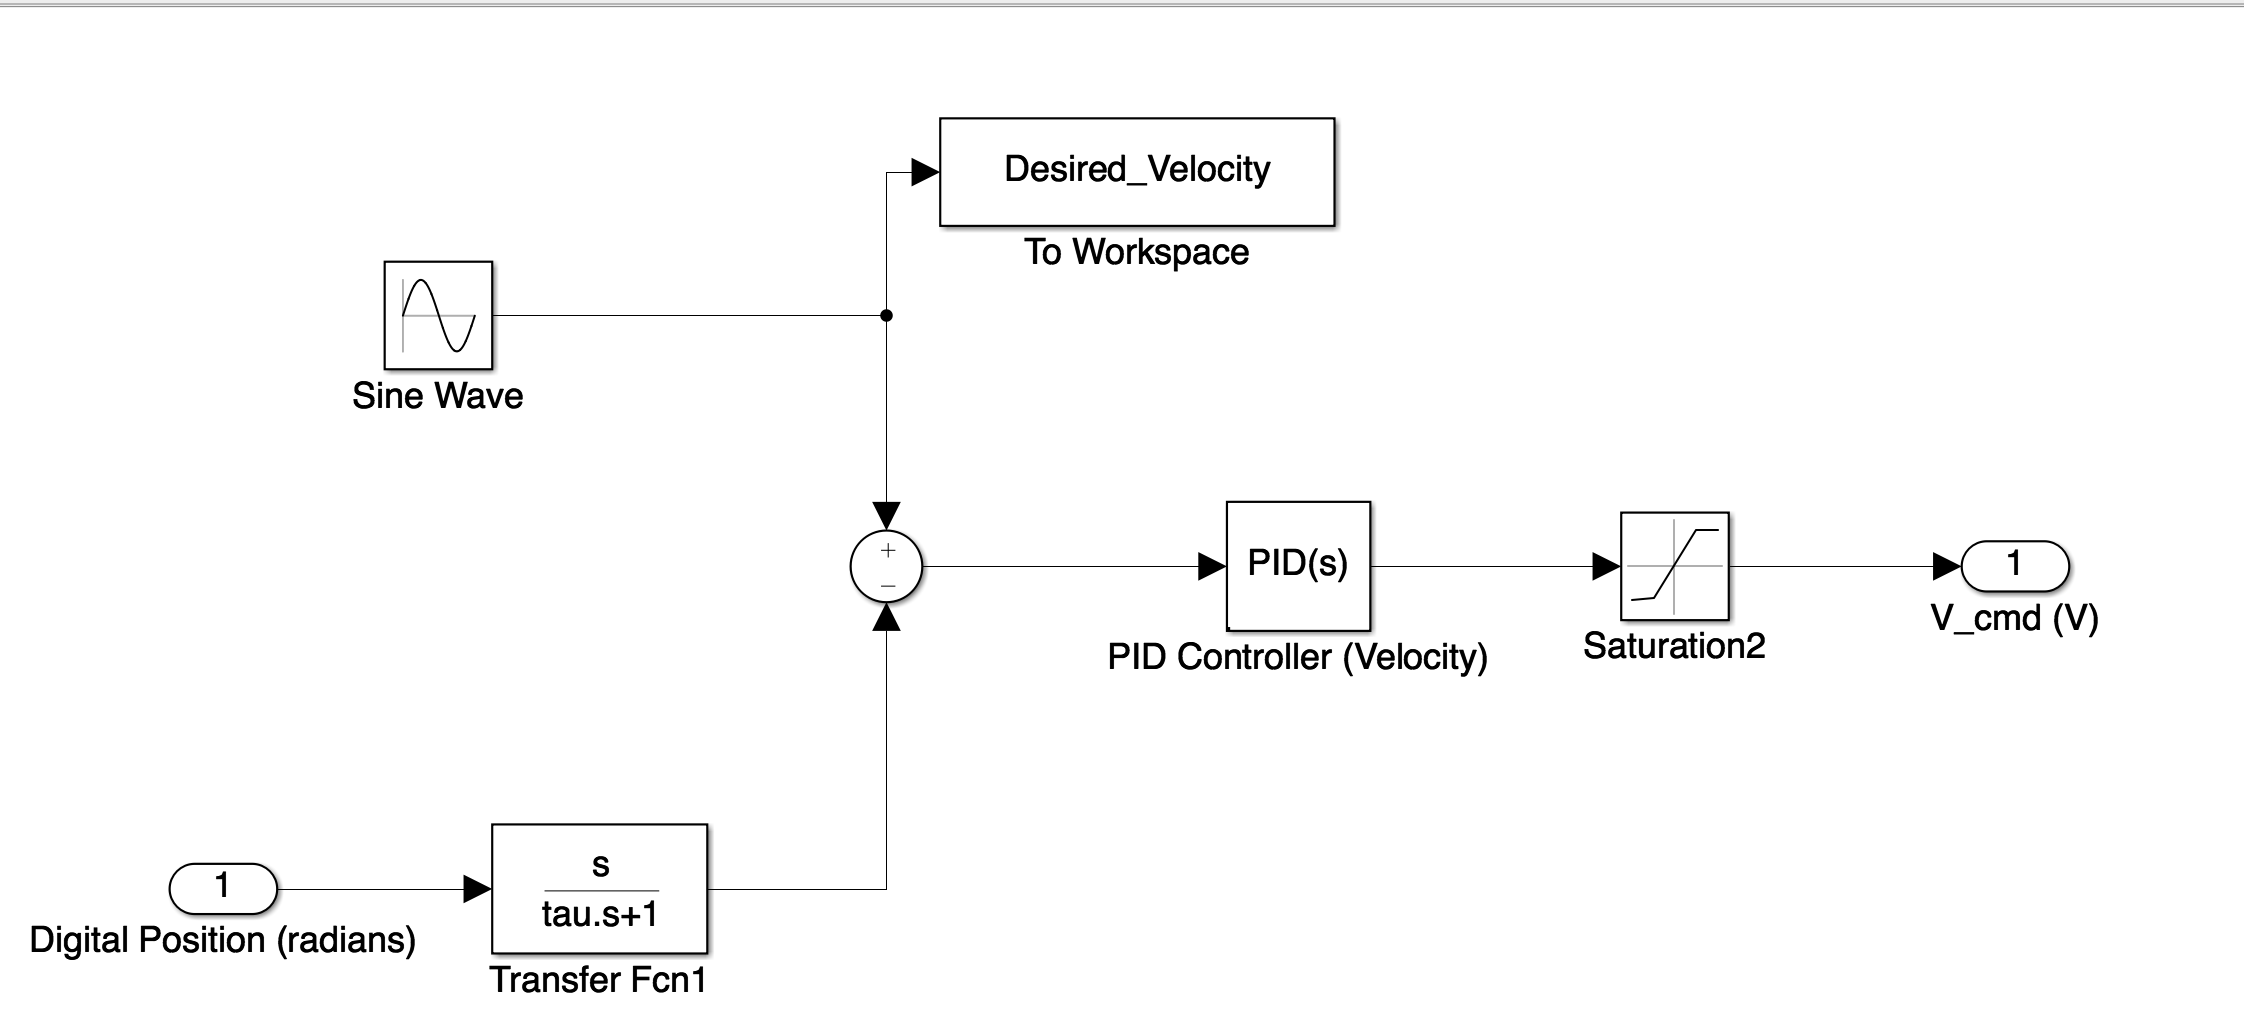
\includegraphics[width = 13cm]{Matlab_simulink_question6.png}
\caption{New controller for velocity control only}
\label{Velocity_control_step}
\end{center}
\end{figure}

Figure \ref{Velocity_control_step} shows the system's response to a velocity step input of 2$\cdot\pi$ radians, and figure \ref{Velocity_control_step_error} shows a zoomed in view after it had settled. The peak error here is even less than 0.001\% (and on average is much less), which greatly satisfies the goal of 2\% error.\\

\begin{figure}[H]
\begin{center}
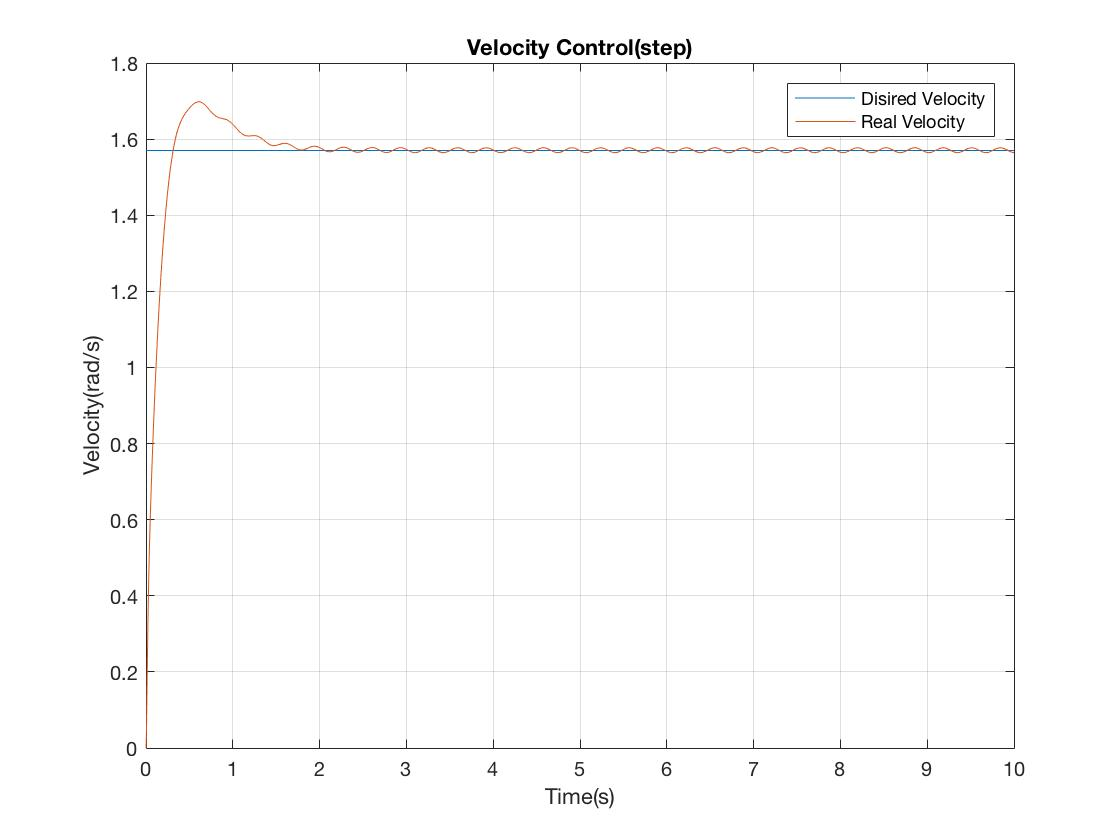
\includegraphics[width = 12cm]{Velocity_control(step).jpg}
\caption{Velocity Controller Step Response}
\label{Velocity_control_step}
\end{center}
\end{figure}

\begin{figure}[H]
\begin{center}
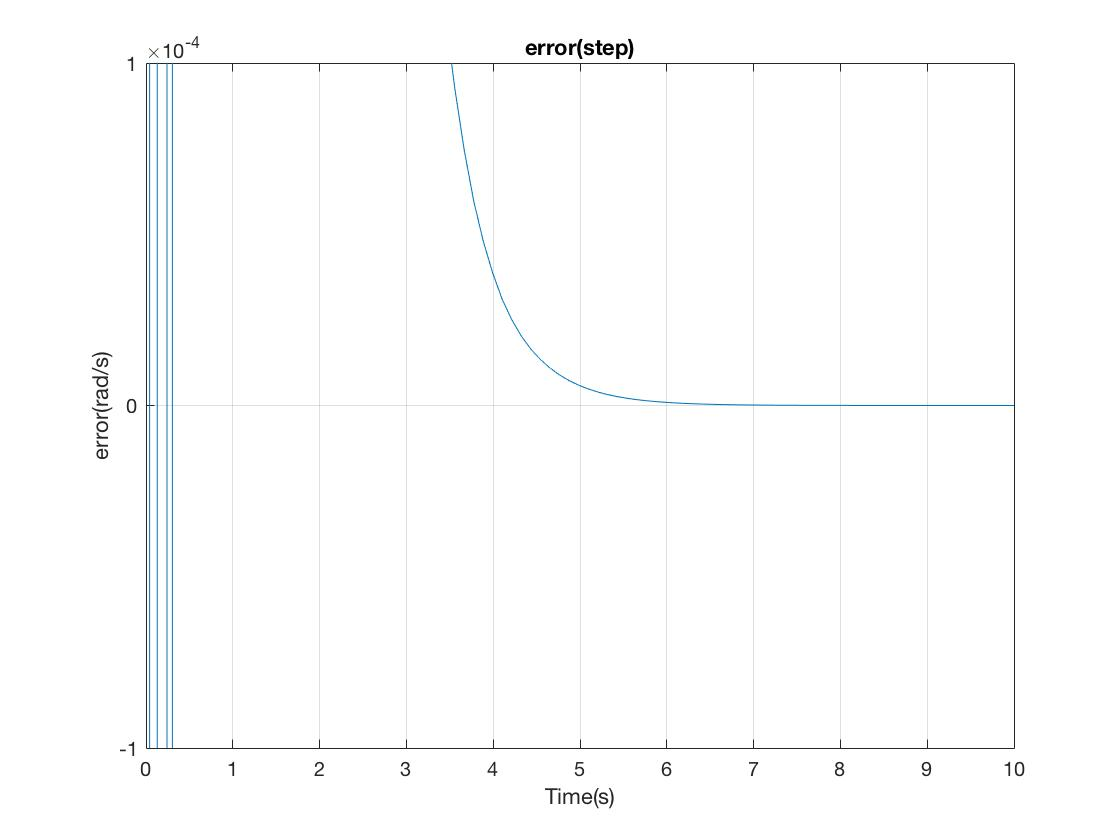
\includegraphics[width = 12cm]{Error(step).jpg}
\caption{Velocity Controller Step Response error}
\label{Velocity_control_step_error}
\end{center}
\end{figure}
%%%%%%%%%%%%%%%加噪音的 step 结果
\subsubsection*{Ideal result for step input with parasitic effects}
Figure \ref{Velocity_control(step)with_parasitic_effects} shows the noise attenuation during a step input of 2$\cdot\pi$ radians/sec. To simulate the noise within Simulink, we added a 60 Hz sine signal with an amplitude of 0.1 to the output of the DAQ assistant. Figure \ref{Error(step)with_parasitic_effects} shows a zoomed in view of steady state error. For the step response with no noise, our peak steady state error was less than 0.0001. Given that we were inputting a noise amplitude of 0.1 and the error only increased by 0.01, we have attenuated the noise by approximately more than 10 times. This meets the goal of a 5 times reduction. Our simulation had an error with noise of 0.16\%, which corresponds to an error of 0.01$rad/s$.\\
\begin{figure}[H]
\begin{center}
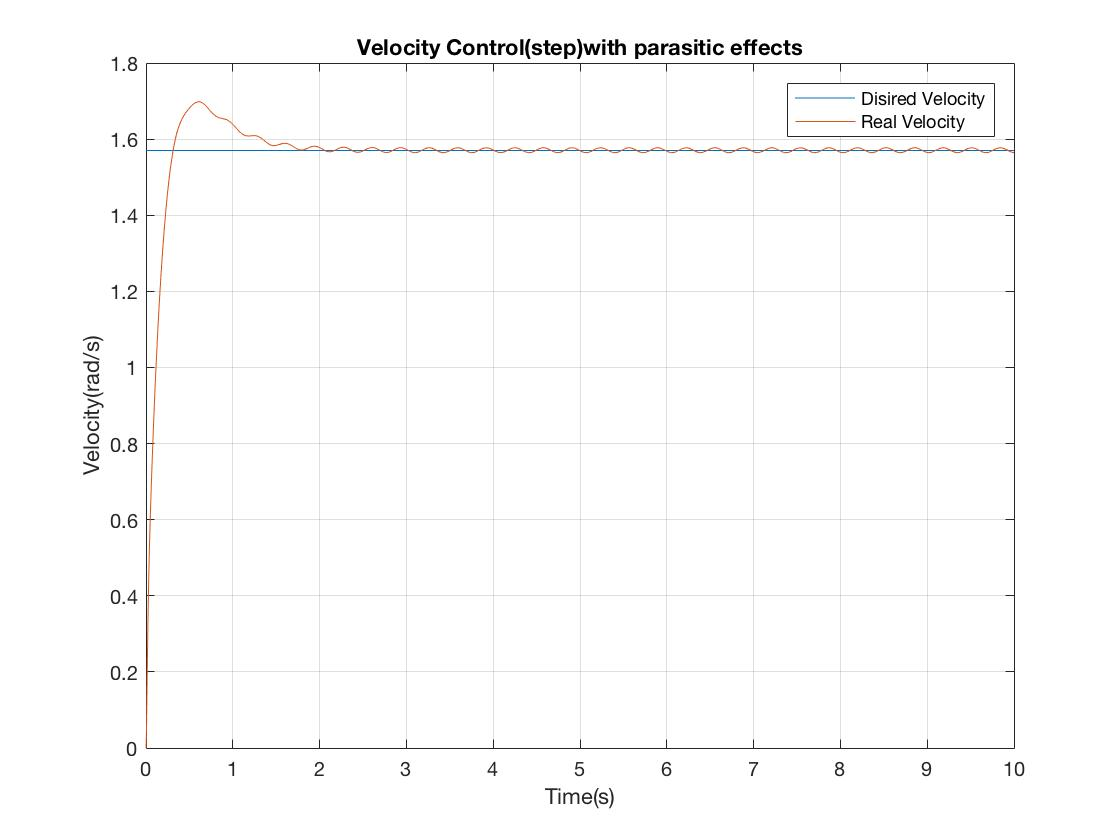
\includegraphics[width = 12cm]{Velocity_control(step)with_parasitic_effects.jpg}
\caption{Velocity Controller Step Response with Parasitic Effects}
\label{Velocity_control(step)with_parasitic_effects}
\end{center}
\end{figure}
\begin{figure}[H]
\begin{center}
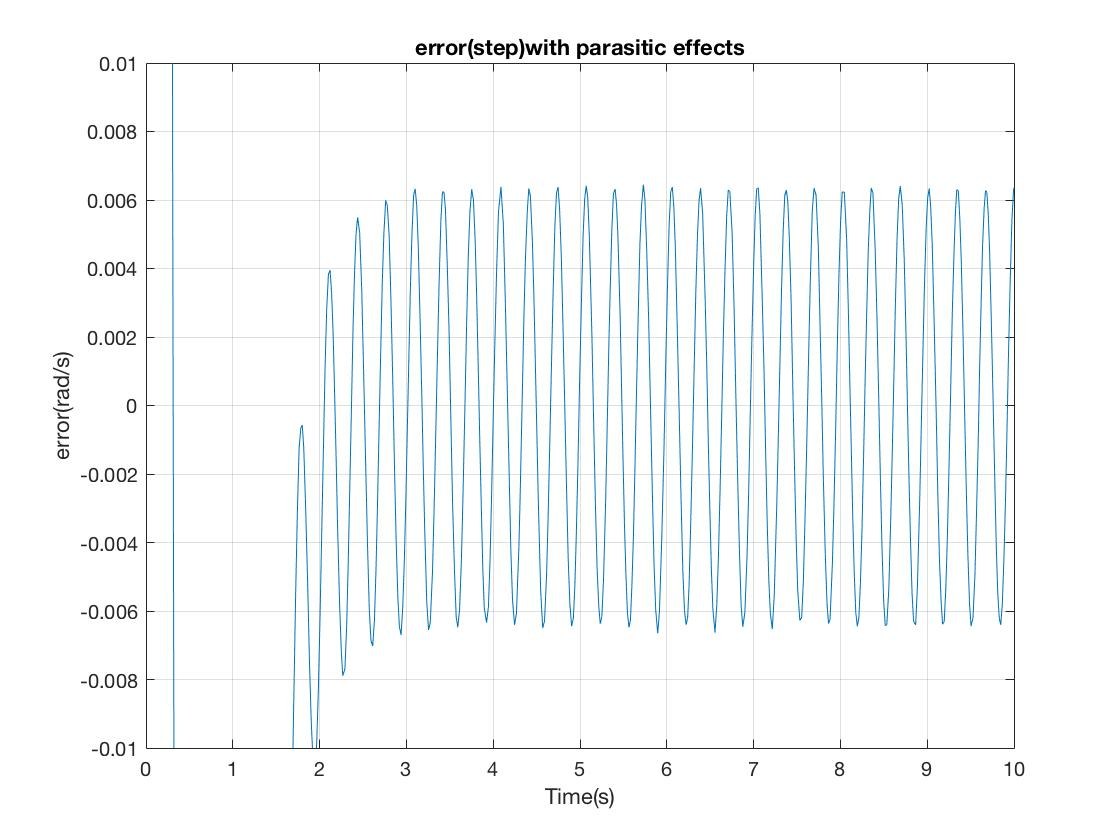
\includegraphics[width = 12cm]{Error(step)with_parasitic_effects.jpg}
\caption{Velocity Controller Step Response Error with Parasitic Effects}
\label{Error(step)with_parasitic_effects}
\end{center}
\end{figure}

\subsubsection*{Experimental result for step input}
%%%%%%%%%%%%%%%实际的 step 结果
While trying the above result on the real physical system, we found that the PID gain of the Simulink result does not work very well. Thus, we slightly adjusted the parameters as shown in Table \ref{velocityGains_step_real}, and the experimental result of which is shown in Figure \ref{velocity_control_step}.\\
\begin{table}[htb]
\begin{center}
    \begin{tabular}{|c|c|c|c|c|}
    \hline
        Gains & P   & I & D     & Filter $\tau$   \\ \hline
        Velocity Controller  & 1.28947 & 2.47423 & 0.025263 & 2.5  \\
    \hline
    \end{tabular}
\end{center}
\caption{Values of velocity controller for real step response}
\label{velocityGains_step_real}
\end{table}

\begin{figure}[H]
\begin{center}
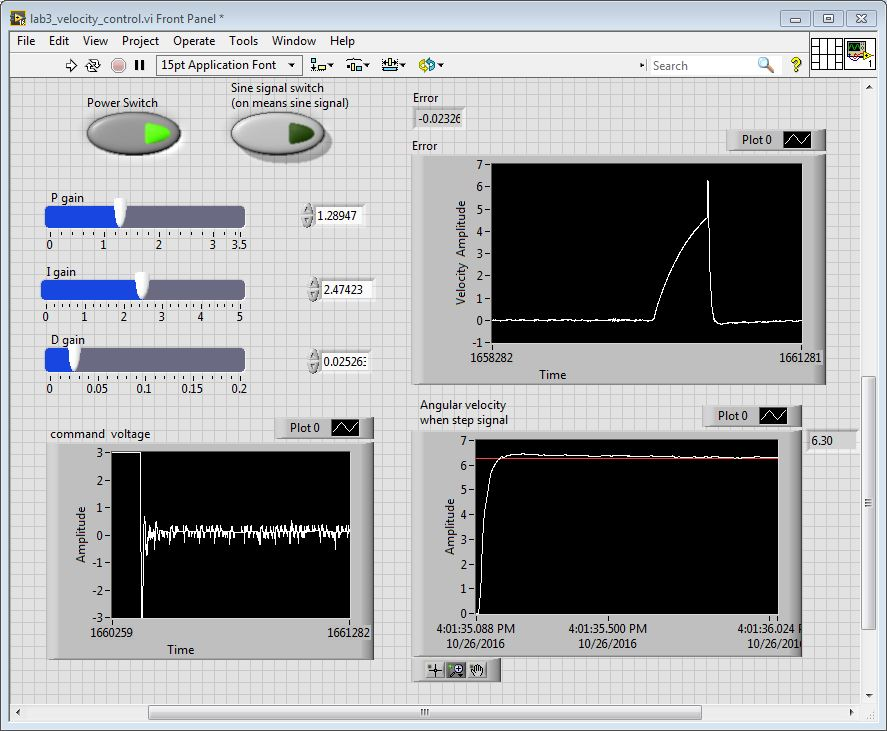
\includegraphics[width = 15cm]{velocity_control_step.JPG}
\caption{Experiment of Velocity Controller Step Response}
\label{velocity_control_step}
\end{center}
\end{figure}

We could see from the above experimental result that the steady state error controlled by the real controller is about 0.02-0.03 $rad/s$ , which is about 0.4-0.5\% error with respect to a total value of $2\pi \ rad/s$. It turns out that the real controller behaves unexpectedly well and satisfied a 2\% error requirement.\\
\subsubsection*{Ideal result for sine signal input}
%%%%%%%%%%%%%%%%理想的 sin 结果
The velocity controller we were using for the step response did not perform well with sinusoidal inputs. Thus, we adjust the PID gain to a different set shown below in Table \ref{velocityGains_sine}.\\
\begin{table}[htb]
\begin{center}
    \begin{tabular}{|c|c|c|c|c|}
    \hline
        Gains & P   & I & D     & Filter $\tau$   \\ \hline
        Velocity Controller  & 25 & 0 & 0.2 & 2.5  \\
    \hline
    \end{tabular}
\end{center}
\caption{Values of velocity controller for ideal sine signal response and noise attenuation}
\label{velocityGains_sine}
\end{table}
\\

Figure \ref{velocity_control_sine} shows the ideal response at frequency equals to $5Hz$ with an amplitude of $\pi$/2. Figure \ref{velocity_control_sine_error} shows the state error with respective to Figure \ref{velocity_control_sine}. From the picture, we may observe that the peak error here is approximately $0.06 rad/s$, which is about 3.8\% (and on average is much less). It satisfies the requirement of 5\% error.\\
\begin{figure}[H]
\begin{center}
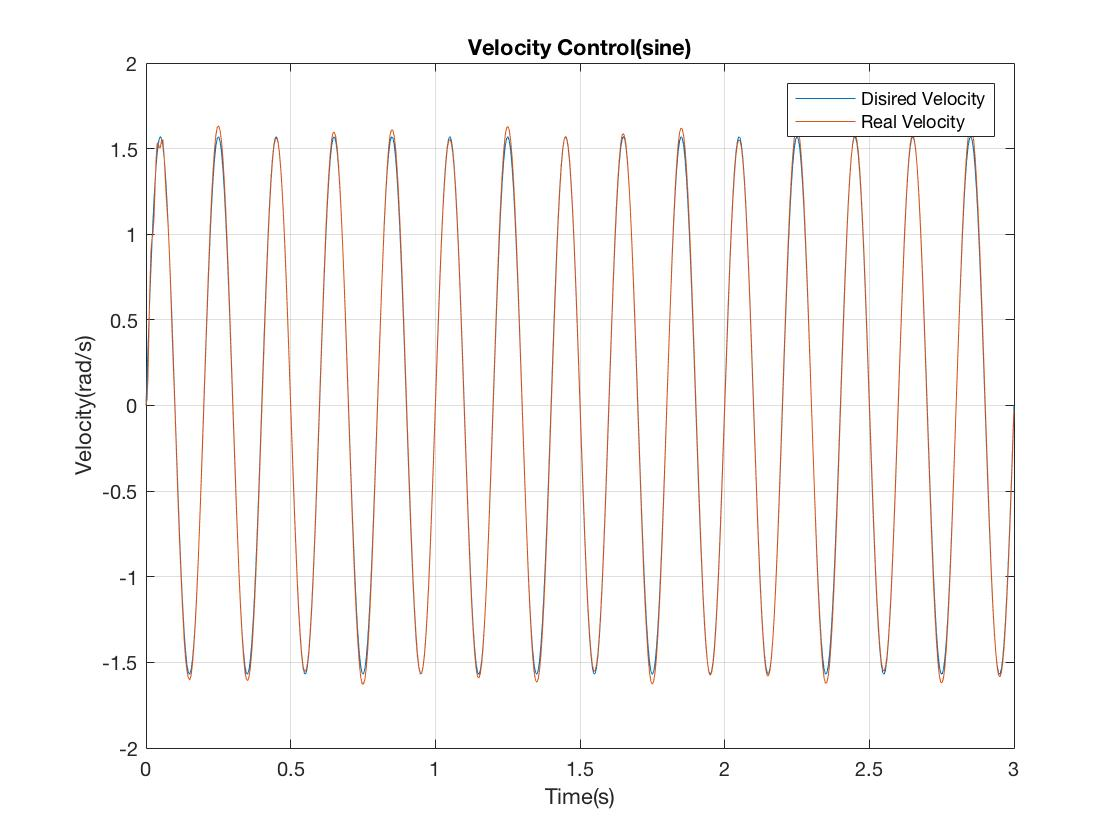
\includegraphics[width = 12cm]{Velocity_control(Sine).jpg}
\caption{Velocity Controller Sine Signal Response}
\label{velocity_control_sine}
\end{center}
\end{figure}

\begin{figure}[H]
\begin{center}
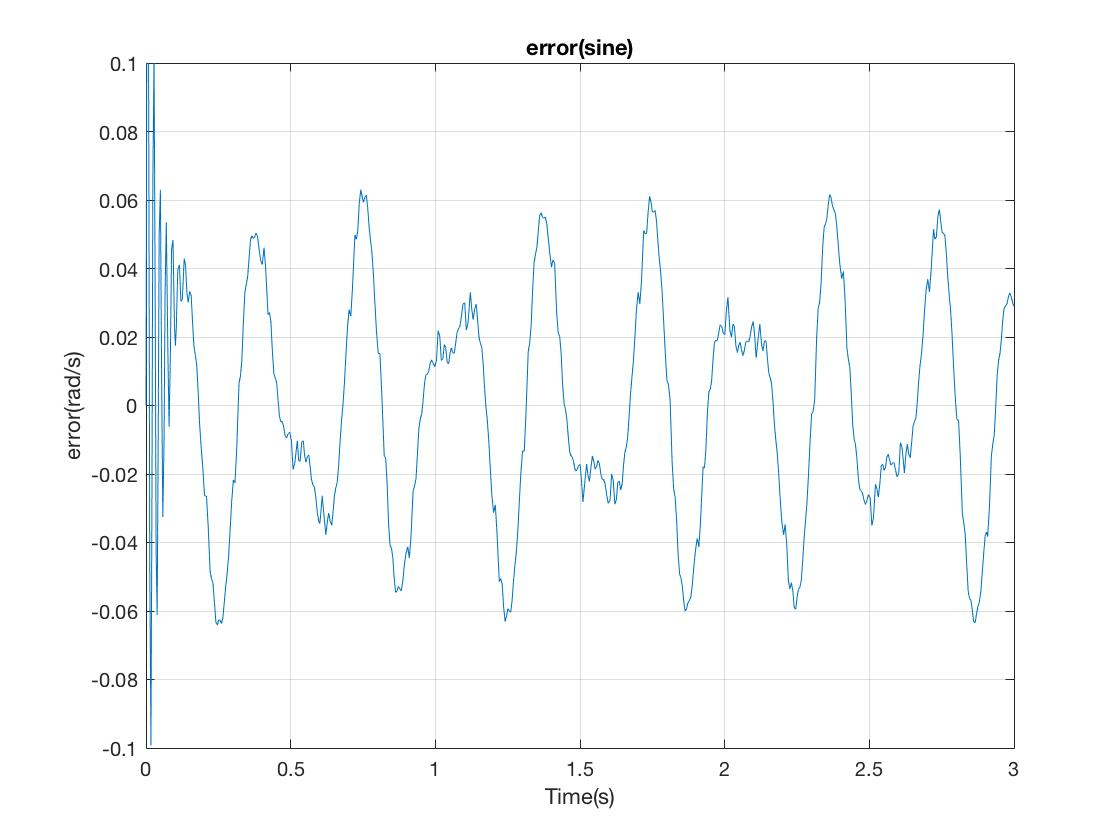
\includegraphics[width = 12cm]{Error(sine).jpg}
\caption{Velocity Controller Sine Signal Error}
\label{velocity_control_sine_error}
\end{center}
\end{figure}
\subsubsection*{Ideal result for sine signal input with parasitic effects}
%%%%%%%%%%%%%%%%%加噪音的 sin 结果
Figure \ref{velocity_control_sine_noise} shows the noise attenuation for a sine signal input of $\pi /2 \ rad/s$. To simulate the noise within Simulink, we added a 60 Hz sine signal with an amplitude of 0.1$rad/s$ to the output of the DAQ assistant. Moreover, we add a friction of $5.6\times 10^{-3} N\cdot m$ as well as the quantization at a rate of 2000 points per circle. Figure \ref{velocity_control_sine_error_noise} shows a zoomed in view of steady state error. For the step response with no noise, our ideal peak steady state error was $0.06 rad/s$, and with the noise the highest error is $0.5 rad/s$.  In all, our simulation had an error with noise of 30\%, which corresponds to an error of $0.5 rad/s$. It still greatly exceeds the goal of 5\% error.\\
\begin{figure}[H]
\begin{center}
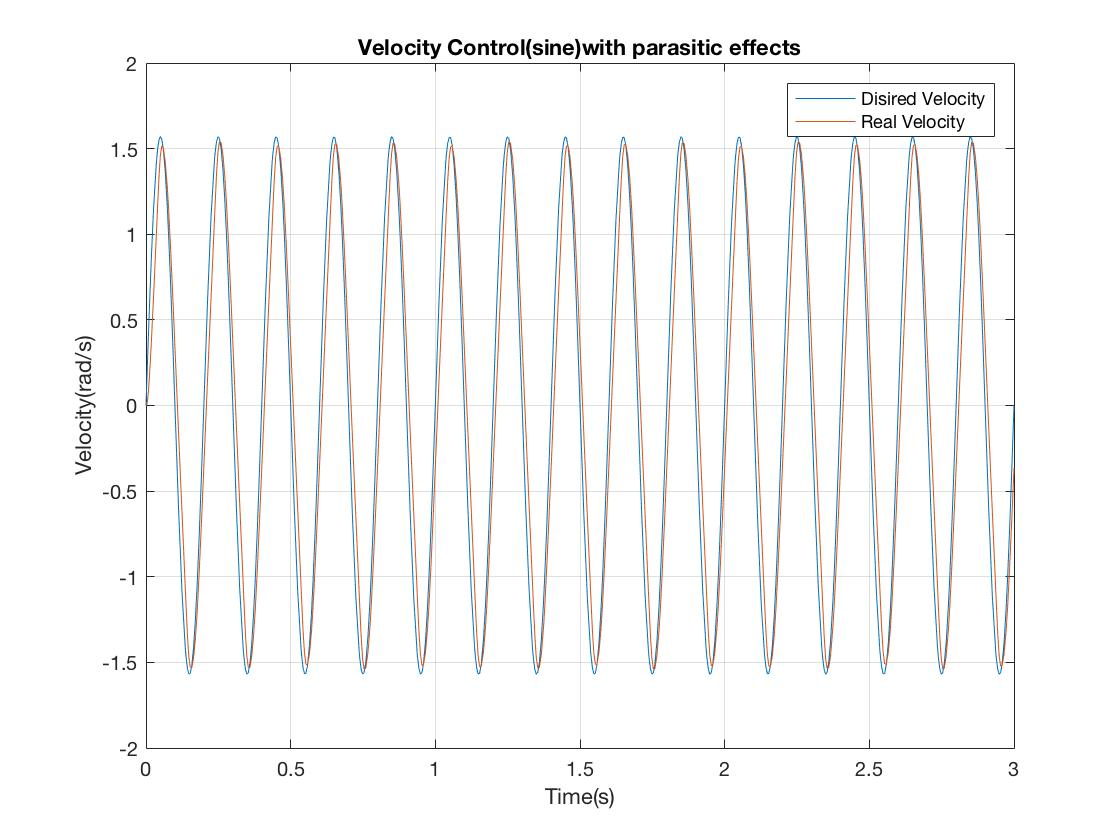
\includegraphics[width = 12cm]{Velocity_control(sine)with_parasitic_effects.jpg}
\caption{Velocity Controller Sine Signal with Parasitic Effects}
\label{velocity_control_sine_noise}
\end{center}
\end{figure}

\begin{figure}[H]
\begin{center}
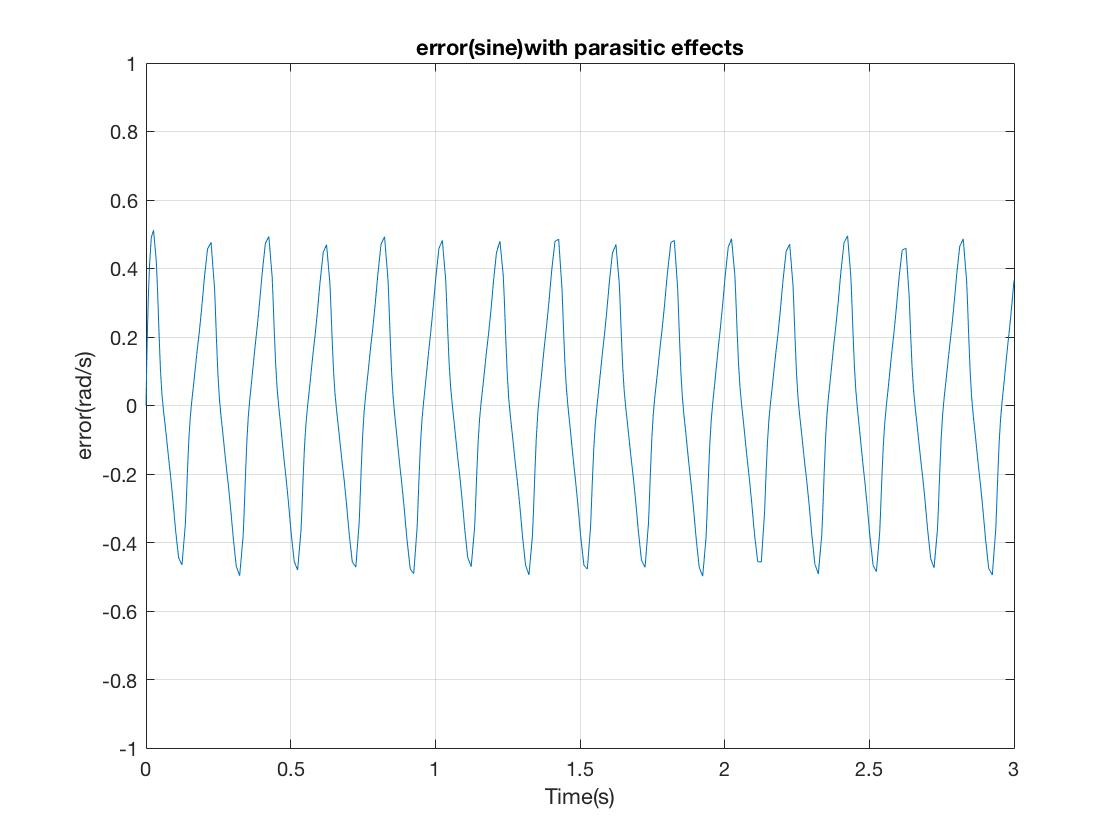
\includegraphics[width = 12cm]{Error(sine)with_parasitic_effects.jpg}
\caption{Velocity Controller Sine Signal Steady Error with Parasitic Effects}
\label{velocity_control_sine_error_noise}
\end{center}
\end{figure}

\subsubsection*{Experimental result for sine signal input}
%%%%%%%%%%%%%%%%%实际的 sin 结果
While trying the above result on the real physical system, we found that the PID gains in Table \ref{velocityGains_sine} behaves in real situations. Instead, we used the same PID gain as of those we used in step input(Table \ref{velocityGains_step_real}), and the experimental result of which is shown in Figure \ref{velocity_control_sine_5hz}.\\
\begin{figure}[H]
\begin{center}
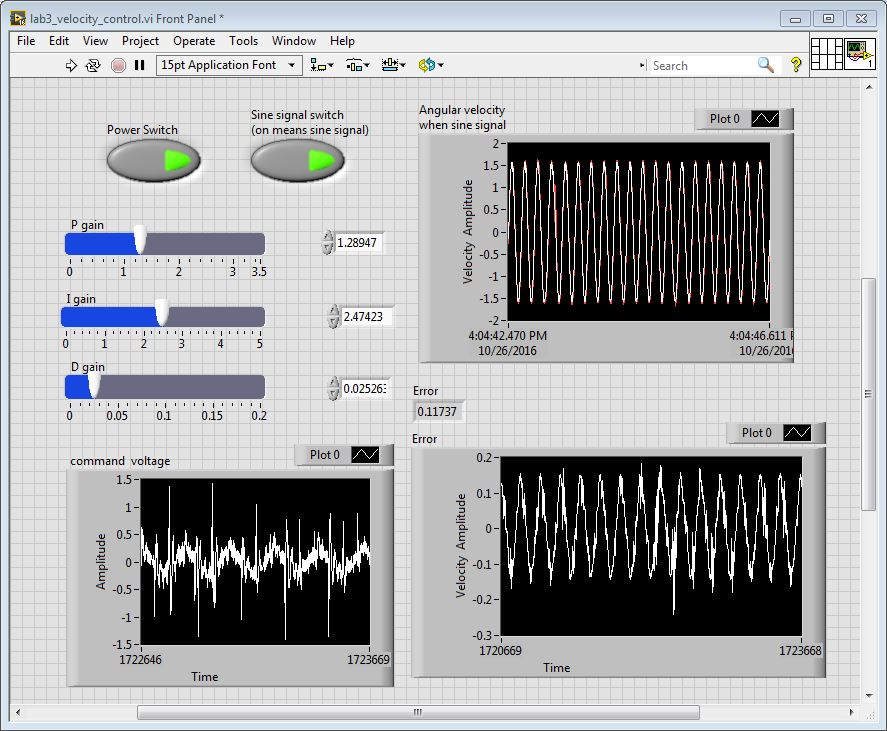
\includegraphics[width = 15cm]{velocity_control_sine_5hz.JPG}
\caption{Experiment of Velocity Controller with Sine Signal Input Amplitude=$\pi/2 \ rad/s$}
\label{velocity_control_sine_5hz}
\end{center}
\end{figure}

We could see from Figure \ref{velocity_control_sine_5hz} that the peak value of steady state error controlled by the real controller is about $0.15 rad/s$ , which is about 10\% steady error with respect to a total value of $\pi /2 \ rad/s$. Apparently, it is not satisfying the requirements of a 5\% error. We tried to adjust the PID gains of the controller, but could not reach to a much improved result. \\

However, we do found the advantages of this controller. While we trying to enlarge the reference signal from $\pi /2 \ rad/s$ to $2\pi \ rad/s$, the state error remain almost the same. As shown in Figure \ref{velocity_control_sine_2pi_5hz}, the input is 4 times larger but the steady state error is only $0.3 rad/s$. Which is to say that the percentage of error is about 5\% of the input signal. In this case, our controller can reach the requirement of a 5\% error. One possible reason which may explain this phenomenon is that we are not reading the real velocity of the motor. Instead, we can only read the velocity after the filter block in Labview, which caused a time delay on the command signal. Thus, there exists an un-eliminate error caused by the delayed command instead of the wrong PID parameters. \\
\begin{figure}[H]
\begin{center}
\includegraphics[width = 15cm]{velocity_control_sine_2pi_5hz.PNG}
\caption{Experiment of Velocity Controller with Sine Signal Input Amplitude=$2\pi \ rad/s$}
\label{velocity_control_sine_2pi_5hz}
\end{center}
\end{figure}
\subsubsection*{Ideal bandwidth}
%%%%%%%%%%%%%%%%%理想的带宽

To determine the closed-loop bandwidth of the system, we slowly increased the frequency of the input signal until the output amplitude just crossed -3 dB (for a input of $\pi$/2 this corresponded to an output of 1.11), just as we did in question 4 to determine the bandwidth of the position controller. We found that the bandwidth of our velocity control system was about 15 Hz, as shown in figure \ref{ideal_bandwith}. \\
\begin{figure}[H]
\begin{center}
\includegraphics[width = 12cm]{15hz.jpg}
\caption{Ideal Bandwith of Velocity Controller}
\label{ideal_bandwith}
\end{center}
\end{figure}

\subsubsection*{Experimental bandwidth}
%%%%%%%%%%%%%%%%%实际的带宽
Then, we implement this 15 Hz frequency into the real velocity control system, the result behaves acceptable, as shown in Figure \ref{real_Bandwidth}. We also noticed that, unlike what we observed in Simulink, the amplitude of the real signal increase as the input frequency increase. The real system behaves so weird may caused by some nonlinear effects which we had not added in our simulation programme. As it is mentioned in question 4 ,it's possible that some of the values used in our simulation are incorrect. At last, we only increase the frequency of the input signal to 15Hz and the steady error reached to $0.6 rad/s$, as shown in Figure \ref{real_Bandwidth}. We tried to increase the frequency of the input signal, but the result behaves even worse. In that case, the ideal bandwidth 15 Hz fits the real bandwidth very well.\\

\begin{figure}[H]
\begin{center}
\includegraphics[width = 15cm]{velocity_control_sine_15hz.JPG}
\caption{Experimental Bandwith of Velocity Controller}
\label{real_Bandwidth}
\end{center}
\end{figure}

Just like with the position controller, we faced a lot of trouble meeting all of the performance specifications with just one controller. One interesting phenomenon which is not mentioned above is that when we adjusted gains to meet the step requirement, the frequency response usually got worse, and vice-versa.In the end we were able to meet the steady state error for step input and noise attenuation requirements, but were not very close to the frequency response requirement.\\

\clearpage



\end{document}
